\documentclass[11pt,a4paper]{article}
\usepackage[margin=2.2cm]{geometry}
\usepackage[T1]{fontenc}
\usepackage{lmodern,microtype}
\usepackage{graphicx,booktabs,tabularx,float,caption,xcolor,enumitem,amsmath,array,multirow}
\usepackage[hidelinks]{hyperref}
\graphicspath{{../figures/}{../../results/plots/}}
\captionsetup{font=small,labelfont=bf}
\setlist{itemsep=2pt,topsep=4pt}
\newcolumntype{R}{>{\raggedleft\arraybackslash}X}
\newcolumntype{L}{>{\raggedright\arraybackslash}X}
\makeatletter % float-only pages: stack floats from the top instead of spreading them out
\setlength{\@fptop}{0pt}\setlength{\@fpsep}{14pt}\setlength{\@fpbot}{0pt plus 1fil}
\makeatother

\title{\textbf{Processing and Visualising Large DEMs on a Laptop}\\[4pt]
\large Final Report}
\author{Team GeoGuessers \quad|\quad Spatial Informatics\\[4pt]
Swayam Goyal (2024111012) \quad Siddharth Choudhary (2024111021)\\
Yakkala Viswanadha Kartikeya (2024111033)}
\date{}

\begin{document}
\maketitle

\begin{abstract}
\noindent
A 1\,m digital elevation model (DEM) of our 100\,km $\times$ 100\,km Himalayan study area holds 10.8 billion cells,
43\,GB as float32, 2.6$\times$ the memory of the laptop we work on. We asked how far such data can be processed and
displayed on one laptop, and which stage actually limits the work. On real DEMs from 90\,m to 2\,m and synthetic 2\,m
and 1\,m grids, we measured the standard tools, built our own terrain engine for the CPU and the GPU, measured the
error and the time saved when derivatives are computed on demand from a pyramid level, and built and measured an
interactive viewer. Six experiments with 2{,}885 separately measured runs and in-process timings give four results.
(1) GDAL's \texttt{gdaldem} never runs out of memory (0.87\,GB at 1\,m) but uses one thread and is compute-bound
(73\% of its time; 3.5\,min for one slope pass at 1\,m); QGIS needs 32\,s to redraw the whole 1\,m area without a
pyramid and 0.09\,s with one. (2) Our tiled engine computes slope 2.1--3.5$\times$ faster than \texttt{gdaldem} on
the same cores, with flat memory (about 1.4\,GB) and results identical to \texttt{gdaldem} on every cell. The GPU
kernel is 50$\times$ faster than the CPU kernel, but a whole run only 1.0--1.4$\times$, because copying data
takes 95\% of the GPU's own time and the run waits for decompression and writing. (3) Computed on demand from the
pyramid, one $512\times512$ display tile costs 5--8\,ms at every zoom level, 8--450$\times$ less than computing it
exactly from full resolution. The price is a systematic underestimate of slope: 2.3$^\circ$ RMSE one level up to
6.4$^\circ$ four levels up on the 2\,m data, worst on steep ground; aspect changes much less. (4) A viewer built on
this keeps up with continuous pan and zoom: 98--100\% of the tiles entering the view while panning are already
cached, a 150\,ms debounce cuts the tiles the server renders per zoom gesture 3.3$\times$, and prefetching does not
slow the visible tiles. On a laptop the limit is moving and decoding data, not arithmetic, so the answer is to read
and compute only what is in view, at the resolution the screen can show.
\end{abstract}

\setcounter{tocdepth}{1}
\makeatletter % compact contents: small gaps between section entries
\let\gg@oldlsection\l@section
\renewcommand*\l@section[2]{{\def\addvspace##1{\vspace{2pt}}\gg@oldlsection{#1}{#2}}}
\makeatother
\tableofcontents
\newpage

%=====================================================================
\section{Introduction}
\subsection{The problem}
A digital elevation model (DEM) is a raster in which every cell stores a ground height. Most terrain analysis starts
from a DEM: GIS tools such as GDAL and QGIS derive slope, aspect, hillshade and roughness from it, as well as
non-local products such as viewsheds and terrain distances. Halving the cell size quadruples the number of cells.
Our study area in the Garhwal Himalaya covers about 100\,km $\times$ 100\,km; at 8\,m it holds 169 million cells,
at 2\,m 2.7 billion and at 1\,m 10.8 billion, or 43\,GB as 4-byte floating-point numbers (float32).

All work in this project runs on one laptop: an Intel Core Ultra 9 185H (6 performance, 8 efficiency and 2 low-power
cores, 22 threads), 16\,GB of RAM, an NVMe SSD and an NVIDIA RTX 4060 Laptop GPU with 8\,GiB of memory, under
Windows 11. A 1\,m grid of our area is 2.6$\times$ larger than the RAM. It cannot be loaded at once, and it cannot be
drawn on a screen at once either: a 1920$\times$1080 screen shows about two million pixels.

\subsection{How the project was framed}
Our first plan was to benchmark slope and aspect algorithms. After a meeting with the course professor the project
was reframed as a systems study. The main points of that meeting were:
\begin{itemize}
  \item Work like a systems team within the hardware we have, and find out how far current DEM tools can be pushed on
  it, with resolutions from about 30\,m down to 1\,m of a Himalayan region.
  \item Do not render the whole dataset. Render only the part the user is looking at, processed on the fly.
  \item Use a pyramid (multi-resolution) representation: coarse levels for large areas, finer levels as the user
  zooms in, so that only the required region and resolution are loaded.
  \item Compute slope and aspect (and, if possible, hillshade, line of sight, viewshed and terrain distance) on demand
  for the region in view, instead of precomputing and storing every derived product.
  \item Do not assume that a GPU is the solution. First find the actual bottleneck (dataset size, CPU or GPU
  computation, memory, CPU--GPU transfer, rendering, loading data), then use the CPU and the GPU where each helps.
  \item Integrate with GDAL and QGIS rather than rebuild a GIS; QGIS and a browser globe such as Cesium are candidate
  viewers.
\end{itemize}
In one sentence: given a very large, high-resolution DEM and limited hardware, process and display only what is
currently needed, using pyramids, on-demand computation and CPU/GPU processing chosen by the measured bottleneck.

\subsection{Research gaps and questions}
Our literature review (Section~\ref{sec:related}) found three gaps:
\begin{itemize}
  \item[\textbf{G1}] No study reports where standard GDAL/QGIS terrain tools stop being practical on a single laptop,
  separated into stages (disk read, computation, CPU--GPU transfer, write, display).
  \item[\textbf{G2}] No study computes terrain derivatives on demand from pyramid levels, or measures the error of
  coarse-level slope against the time it saves.
  \item[\textbf{G3}] The accuracy loss of fast approximate viewsheds (XDraw) against the exact R3 method in
  high-relief terrain, and A* against Dijkstra for terrain distance. This was a stretch goal and is left as future
  work.
\end{itemize}
From G1 and G2 and the meeting we derived four questions:
\begin{enumerate}
  \item[\textbf{Q1}] Where do the standard tools stop being practical, and which stage limits them? (G1)
  \item[\textbf{Q2}] Once computation is parallel, on the CPU or the GPU, where does the bottleneck move, and when
  does a GPU help? (G1)
  \item[\textbf{Q3}] How wrong is slope computed from a coarse pyramid level, and how much time does it save? (G2)
  \item[\textbf{Q4}] Can on-demand computation support continuous pan and zoom on the laptop, and with which policy?
\end{enumerate}

\subsection{Contributions}
\begin{enumerate}
  \item A measurement harness and protocol for a hybrid-core Windows laptop: exact per-process time, memory, CPU and
  I/O, a verified cold file cache, pinning to performance cores, and control of background interference.
  \item A stage-by-stage baseline of \texttt{gdaldem} and QGIS from 1.3 million to 10.8 billion cells (E1, E2, QGIS
  display; 832 runs).
  \item An out-of-core terrain engine for the CPU (Numba) and the GPU (our own CUDA kernels) that reproduces all ten
  \texttt{gdaldem} operator configurations, verified on every cell of four full real grids, and a measurement of how
  the bottleneck moves once computation is parallel (E3, E4; 985 runs).
  \item A measurement on real data of the slope and aspect error of every pyramid level against the time saved, by
  terrain class, with a comparison against independent DEMs (E5, gap G2).
  \item A working viewer system (tile engine, scheduler, server, web viewer and QGIS plugin) whose policy (debounce,
  prefetch, worker placement, caches) was set from 1{,}068 measured runs (E6).
\end{enumerate}
Section~\ref{sec:related} reviews related work, Section~\ref{sec:data} describes the data and
Section~\ref{sec:method} the benchmark method. Sections~\ref{sec:baseline}--\ref{sec:viewer} present the
experiments E1--E6. Section~\ref{sec:discussion} brings the results together, and Section~\ref{sec:conclusion}
concludes.

%=====================================================================
\section{Related work}\label{sec:related}
This section summarises the team's literature review of sixteen studies, grouped into four themes.

\paragraph{Local terrain operators.} Slope, aspect, hillshade and curvature are computed from a $3\times3$ window
around each cell. Horn \cite{horn} weights the four direct neighbours twice as heavily as the diagonal ones;
Zevenbergen and Thorne \cite{zt} fit a surface through the window, from which curvature also follows. GDAL uses
Horn's method by default and offers Zevenbergen--Thorne as an option. Guth and Kane \cite{guth} adapted slope, aspect
and hillshade to non-square cells and found that computed slope changes roughly logarithmically with grid spacing.
The terrain ruggedness index (TRI) has two common forms (Riley et al.\ \cite{riley}, Wilson et al.\ \cite{wilson});
Trevisani et al.\ \cite{trevisani} revisited it and proposed a radial roughness index. Every operator in this group
visits each cell once and costs $O(N)$ for $N$ cells, so a naive and a state-of-the-art version share the same
complexity and differ only in implementation.

\paragraph{Resolution and data volume.} Zhang and Montgomery \cite{zhang} showed long ago that computed slope
decreases as the grid becomes coarser. Deng et al.\ \cite{deng} found that the change depends on the position of a
point in the landform, and Polidori and El Hage \cite{polidori} argue that source errors propagate into every
derivative, so nominal resolution is a weak guide to a DEM's usefulness. Global products show the cost side:
Amatulli et al.\ \cite{amatulli} computed geomorphometric layers for the whole globe, and Ho et al.\ \cite{ho} note
that a 1 arc-second global grid holds about 202 billion pixels and can only be processed by tiling with overlap, in
parallel. Both precompute every layer at fixed scales.

\paragraph{Scaling computation.} Barnes \cite{barnes} tiled the DEM in a producer--consumer scheme that runs
unchanged on one core, many cores or a cluster, and reached trillion-cell datasets on ordinary hardware. Yu et al.\
\cite{yu} scheduled neighbourhood operations on the CPU and the GPU together and reached a speed-up of about 29 on a
1.7\,GB raster, a fifth better than with the GPU alone. For non-local operations the methods do differ in
complexity: the exact R3 viewshed costs $O(N^{1.5})$ and the approximate XDraw $O(N)$
\cite{sanchez}. XDraw has been mapped to the GPU \cite{cauchi} and load-balanced over equal-area partitions
\cite{dou}, and Sanchez-Fernandez et al.\ \cite{sanchez} showed that restructuring the DEM in memory mattered more
than adding GPUs. For terrain distance, A* with an admissible heuristic finds the optimal path while expanding fewer
nodes than Dijkstra's search \cite{hart}.

\paragraph{Display.} Losasso and Hoppe \cite{clipmaps} cache terrain in nested grids centred on the viewer, so that
detail follows the view at a steady frame rate whatever the dataset size. Campos et al.\ \cite{campos} built a
multi-resolution pyramid for virtual globes one tile at a time, because a continent-scale mesh does not fit in
commodity memory, and displayed it in Cesium. These pyramids carry elevation only: derived products are still
computed in advance.

\paragraph{What is missing.} The studies agree that tiling with overlap is the accepted way to handle grids larger
than memory, and that data movement usually limits performance more than arithmetic. Reported speed-ups range from
29 to over 800 times across different baselines and hardware, and no study separates disk read, CPU--GPU transfer,
computation and display, so it is unclear when a GPU helps (G1). Pyramids are used for display, but nobody computes
derivatives from them on demand or measures the resulting error against the time saved (G2). A pilot test for the
review, run through the QGIS interface on a different laptop, saw a roughly threefold difference between first and
repeated slope runs at 5\,m, which suggested that file caching dominates. Section~\ref{sec:baseline} revisits that
pilot under a controlled protocol.

%=====================================================================
\section{Data and study area}\label{sec:data}
\subsection{One area, many resolutions}
Run time depends on the number of cells, not on which mountain is processed. All experiments therefore use one
study area, so that grid size is the only variable that changes (Figure~\ref{fig:area}, Table~\ref{tab:data}). The
area is NASA High Mountain Asia (HMA) tile-571 in the Garhwal Himalaya (Uttarakhand, Nanda Devi region),
79.125--80.235$^\circ$E and 30.033--30.970$^\circ$N, with elevations from 674 to 7{,}790\,m. Inside it lies the
Chamoli (Rishiganga) sub-area, about 30\,km $\times$ 35\,km, covered by a real 2\,m DEM.

\begin{figure}[!htbp]
\centering
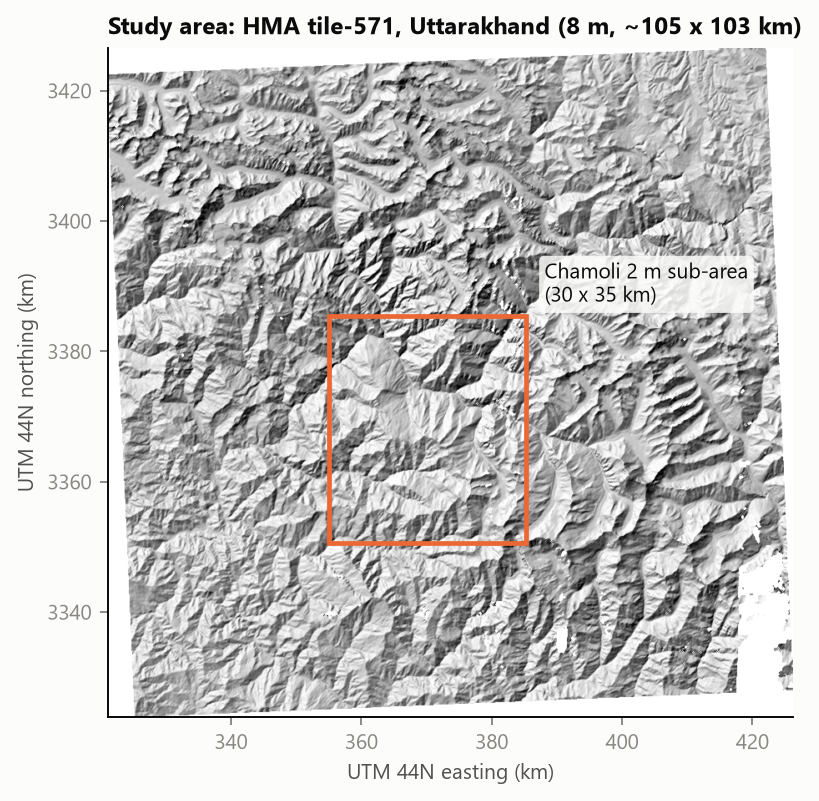
\includegraphics[width=0.5\linewidth]{study_area.png}
\caption{Study area (shaded relief of the 8\,m DEM) and the Chamoli sub-area covered by the real 2\,m DEM.}
\label{fig:area}
\end{figure}

\begin{table}[!htbp]
\centering\small
\caption{Resolution ladder. Real grids are used for timing and accuracy, synthetic grids only for timing.}
\label{tab:data}
\begin{tabularx}{\linewidth}{lllrrL}
\toprule
Res. & Source & Type & Cells & Valid & Role \\
\midrule
90\,m & Copernicus GLO-90 (OpenTopography) & real & 1.3\,M & 100\% & coarsest level \\
30\,m & Copernicus GLO-30 \cite{cop30} & real & 12\,M & 100\% & baseline level \\
8\,m & HMA 8\,m mosaic, tile-571 \cite{hma8} & real & 169\,M & 84\% & finest real, whole area \\
2\,m & Chamoli 2\,m composite \cite{chamoli} & real & 264\,M & 94\% & accuracy truth (sub-area) \\
2\,m & cubic upsample of 8\,m & synthetic & 2.7\,B & $\sim$89\% & timing only \\
1\,m & cubic upsample of 8\,m & synthetic & 10.8\,B & $\sim$89\% & timing only; 43\,GB \\
\bottomrule
\end{tabularx}
\end{table}

\subsection{Preparation and checks}
All grids were reprojected to WGS\,84 / UTM zone 44N (EPSG:32644), so that cell sizes are true metres, on one
aligned grid: every grid shares one origin on a 360\,m lattice, which is divisible by 90, 30, 8, 2 and 1. Each grid
is stored as a Cloud-Optimized GeoTIFF (COG): a GeoTIFF in $512\times512$ tiles with ZSTD compression and internal
overviews. An overview is a coarser copy of the grid stored in the same file; the overviews, built by GDAL with
averaging, form the pyramid that a viewer reads. Level $k$ has a cell size of about $2^k$ times the base cell (on the
2\,m data: 4, 8, 16, 32, 64 and 128\,m).

\begin{itemize}
  \item \textbf{Agreement between sources.} All downloads were checksum-verified. Where the 2\,m and 8\,m DEMs
  overlap, the 2\,m DEM averaged to 8\,m minus the 8\,m DEM has a median of $-0.7$\,m and an NMAD (normalised median
  absolute deviation, a robust standard deviation) of 5.1\,m over 14 million cells. The 8\,m DEM sits 24.5\,m below
  Copernicus, because HMA heights refer to the WGS\,84 ellipsoid and Copernicus heights to the EGM2008 geoid. A
  near-constant offset does not affect slope, aspect or hillshade.
  \item \textbf{Synthetic grids.} No free 1\,m DEM exists for this region, so the 2\,m and 1\,m grids of the whole
  area are cubic upsamples of the 8\,m tile. To test how reliable such grids are, an 8\,m crop of 16 million cells
  was rebuilt from a 16\,m version of itself. It gave the same \texttt{gdaldem} run time as the real crop
  (0.87--0.90\,s) but 2.3--3.0$^\circ$ slope RMSE against it. Synthetic grids are therefore used for timing only.
  Cubic resampling was chosen because nearest-neighbour data compresses 26\% better than real terrain and would make
  reads look faster than they are.
\end{itemize}

%=====================================================================
\section{Benchmark method}\label{sec:method}
\paragraph{Software.} GDAL 3.13.3 and QGIS 3.44.14 as the baseline; our engine in Python with Numba \cite{numba}
for the CPU and CuPy \cite{cupy} (CUDA 12.9) for the GPU; FastAPI for the viewer's server.

\paragraph{Harness.} Each measurement runs one tool as a separate process. When the process ends, the harness reads
from Windows, for that process only, its wall time, peak memory (peak working set), CPU time and bytes read and
written, and it counts the bytes physically read from disk. CPU time divided by wall time gives the average number
of threads used. Our engine also reports its own stage timings. Every run is one row in a results table, with the
dataset, operator, method, cache state and code version; sweeps can be resumed.

\paragraph{Protocol.}
\begin{itemize}
  \item \textbf{Cold and warm cache.} Before every cold run, the Windows file cache (standby list) is emptied with
  Sysinternals RAMMap through a scheduled task; we verified that the whole file is then read from disk again. A warm
  run is an immediate repeat.
  \item \textbf{Repeats.} Real grids: 5 cold runs, then 1 warm-up and 5 warm runs. Synthetic 2\,m and 1\,m grids:
  3 cold runs and 1 warm run. Medians are reported, and the median and interquartile range (IQR) of every
  configuration are kept. The median IQR is 1.4\% of the median for E1, 1.3\% for E2, 1.6\% for the QGIS runs,
  1.6\% for E3 and 1.2\% for E4.
  \item \textbf{Core pinning.} \texttt{gdaldem} runs 1.7$\times$ slower on an efficiency core and up to 2.7$\times$
  slower on a low-power core, and Windows can move a process between them during a run: one unpinned run took
  108.9\,s instead of about 56\,s. All tools are therefore pinned to the 12 performance-core threads, i.e.\ measured
  at their best. Our engine was measured both on these 12 threads and on all 22.
  \item \textbf{Background activity.} Windows Defender scanning our 10--40\,GB temporary outputs held disk space and
  slowed later runs by 25--35\%. Only the two scratch folders were excluded from scanning, the harness waits until
  deleted outputs are released before the next run, and all final numbers were re-run under these conditions.
  Earlier, disturbed attempts are kept as evidence.
  \item \textbf{Stage split.} For each grid, two reference runs split a \texttt{gdaldem} run into stages: a pure read
  and decompress of every block, and a copy to an uncompressed GeoTIFF (the same read and the same-size write).
  Then write $\approx$ copy $-$ read, and compute $\approx$ \texttt{gdaldem} $-$ copy.
\end{itemize}
Sizes use MB $=10^6$ and GB $=10^9$ bytes; GPU and client memory are given in MiB and GiB.

\begin{table}[!htbp]
\centering\small
\caption{The six experiments. E5 runs inside one long-lived process (as a viewer's server would); the others run
every measurement as a separate process.}
\label{tab:experiments}
\begin{tabularx}{\linewidth}{llLr}
\toprule
ID & Question & What was varied & Runs \\
\midrule
E1 & How does \texttt{gdaldem} scale? & 10 operator configurations, 6 grids, cold/warm & 560 \\
E2 & Does storage layout matter? & 7 layouts (strips/tiles, 256/512, none/LZW/DEFLATE/ZSTD) & 224 \\
QGIS & What limits display? & whole area / zoomed in, with / without pyramid, 3 grids & 48 \\
E3 & How fast is our CPU engine? & 24 variants: threads, operators, fused products, windows, naive & 501 \\
E4 & When does the GPU help? & optimisation steps, precision, operators, windows, readers; crossover & 484 \\
E5 & Error vs time on the pyramid & every pyramid level of two real DEMs; three routes per view & in-process \\
E6 & Does the viewer keep up? & 24 configurations $\times$ 17 interaction traces & 1{,}068 \\
\bottomrule
\end{tabularx}
\end{table}

%=====================================================================
\section{Where standard tools stop being practical (E1, E2, QGIS)}\label{sec:baseline}
\subsection{E1: \texttt{gdaldem} across grid sizes}
\texttt{gdaldem} is GDAL's terrain tool; QGIS's slope, aspect and hillshade tools call it. E1 ran its ten operator
configurations (slope, aspect and hillshade with Horn and Zevenbergen--Thorne, TRI after Riley and Wilson, TPI and
roughness) on all six grids, cold and warm (Table~\ref{tab:e1}, Figure~\ref{fig:e1}).

\begin{table}[!htbp]
\centering\small
\caption{\texttt{gdaldem} (Horn) by grid size. Medians; ns per cell for slope, warm cache.}
\label{tab:e1}
\begin{tabularx}{\linewidth}{lRRRRRRR}
\toprule
Grid & Cells & Slope cold & Slope warm & Hillshade warm & ns/cell & Peak memory & Threads used \\
\midrule
90\,m & 1.3\,M & 0.08\,s & 0.07\,s & 0.06\,s & (start-up) & 42\,MB & 0.88 \\
30\,m & 12\,M & 0.29\,s & 0.28\,s & 0.13\,s & 23.1 & 96\,MB & 0.97 \\
8\,m & 169\,M & 4.10\,s & 4.02\,s & 2.96\,s & 23.8 & 745\,MB & 0.98 \\
2\,m real & 264\,M & 6.67\,s & 6.63\,s & 4.74\,s & 25.1 & 868\,MB & 0.99 \\
2\,m synth. & 2.7\,B & 54.2\,s & 53.7\,s & 41.0\,s & 19.9 & 870\,MB & 0.99 \\
1\,m synth. & 10.8\,B & 208.3\,s & 208.4\,s & 158.9\,s & 19.3 & 872\,MB & 0.99 \\
\bottomrule
\end{tabularx}
\end{table}

\begin{figure}[!htbp]
\centering
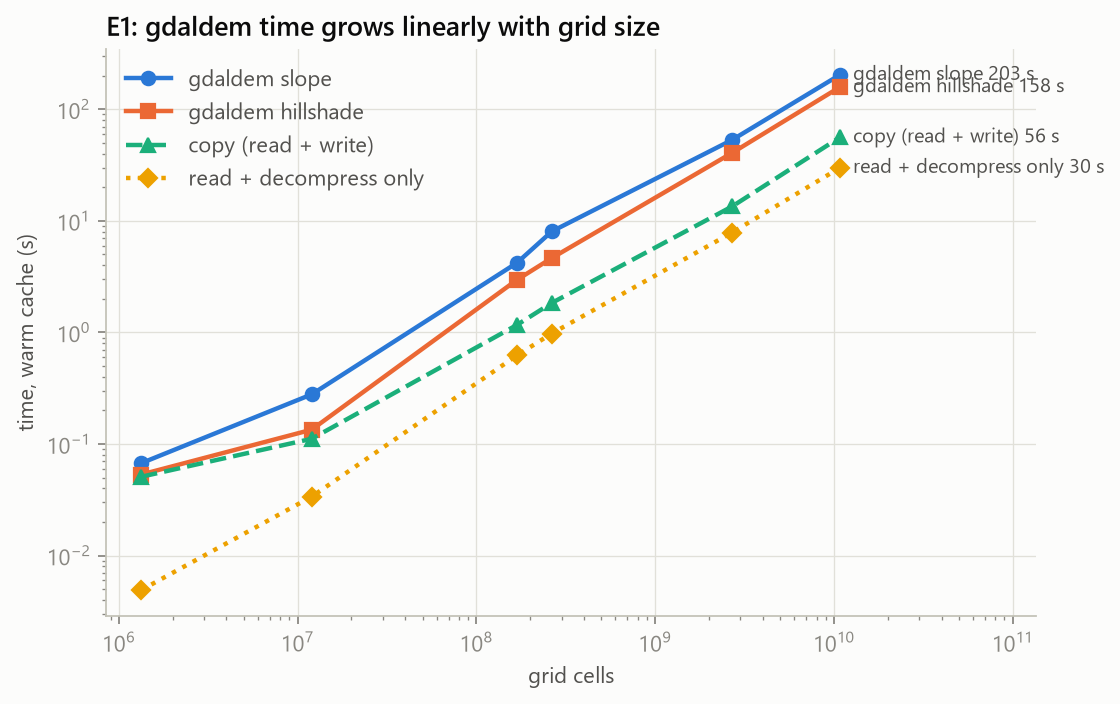
\includegraphics[width=0.49\linewidth]{e1_scaling.png}\hfill
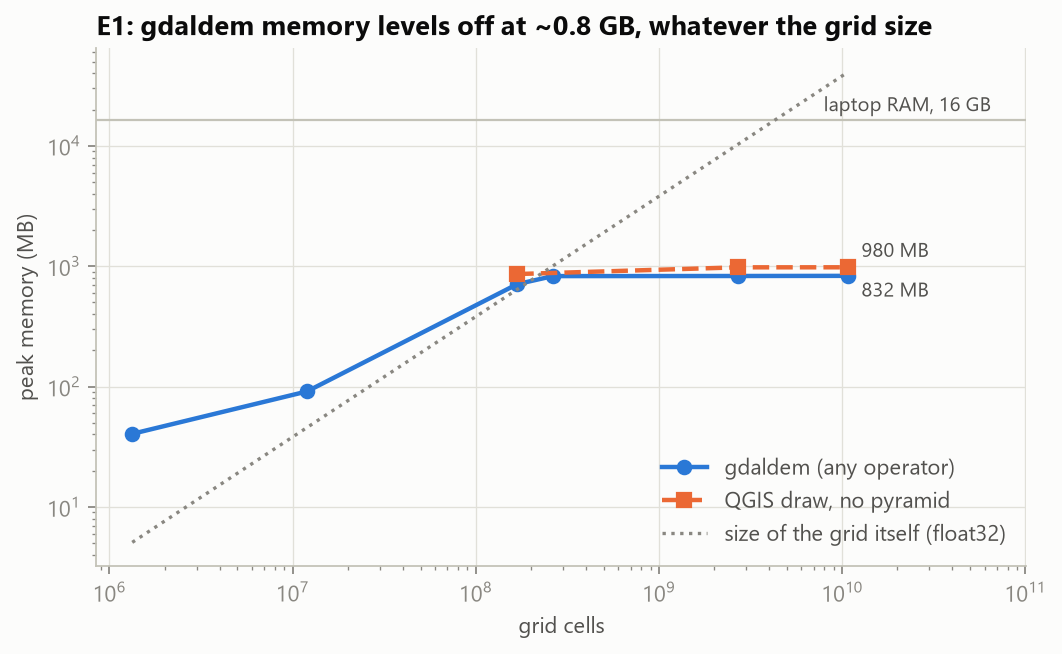
\includegraphics[width=0.49\linewidth]{e1_memory.png}
\caption{E1. Left: \texttt{gdaldem} run time grows linearly with the number of cells. Right: peak memory levels off
at about 0.87\,GB, far below the size of the grid, which exceeds the 16\,GB RAM at 1\,m.}
\label{fig:e1}
\end{figure}

\begin{itemize}
  \item \textbf{No memory limit.} \texttt{gdaldem} streams the grid in strips and processes 43\,GB of data with a peak
  of 0.87\,GB, about GDAL's default block cache (5\% of RAM) plus the program.
  \item \textbf{Linear time.} Once program start-up stops mattering (above about 10 million cells), slope costs
  19--25\,ns per cell: 3.5\,min for one slope pass over the 1\,m grid.
  \item \textbf{One thread.} \texttt{gdaldem} uses 0.99 of 22 threads at every large size.
  \item \textbf{The file cache does not matter.} Cold and warm runs differ by 2\% or less. At 2\,m and 1\,m even warm
  runs read 3.8 and 14.2\,GB from disk (the 1\,m file does not fit in the cache; at 2\,m the $\sim$11\,GB that
  \texttt{gdaldem} writes pushes the input out) and take the same time.
\end{itemize}

\begin{table}[!htbp]
\centering\small
\caption{Where \texttt{gdaldem}'s slope time goes (stage split, warm references).}
\label{tab:stages1}
\begin{tabularx}{\linewidth}{lRRR}
\toprule
Grid & Read + decompress & Write + tool overhead & Compute \\
\midrule
8\,m & 15\% (0.61\,s) & 14\% (0.57\,s) & 71\% (2.83\,s) \\
2\,m real & 15\% (0.99\,s) & 11\% (0.76\,s) & 74\% (4.88\,s) \\
2\,m synthetic & 15\% (7.9\,s) & 11\% (6.2\,s) & 74\% (39.7\,s) \\
1\,m synthetic & 14\% (29.0\,s) & 13\% (26.8\,s) & 73\% (152.6\,s) \\
\bottomrule
\end{tabularx}
\end{table}

\paragraph{Where the time goes.} About 73\% of every large run is single-threaded computation, 14--15\% reading and
decompressing and 11--14\% writing (Table~\ref{tab:stages1}). The ten operators cost 17.5--27\,ns per cell on the
2\,m real grid: TPI is the cheapest, and slope and aspect, which need trigonometric functions, are the most
expensive. Horn and Zevenbergen--Thorne differ by at most 6\% (slope 4\%, aspect 6\%, hillshade 0\%), so the choice
of formula is not where speed comes from.

\paragraph{Is the baseline configured fairly?} GDAL can decompress tiles in parallel (\texttt{GDAL\_NUM\_THREADS})
and enlarge its block cache (\texttt{GDAL\_CACHEMAX}). With parallel decoding \texttt{gdaldem} used about two cores
but ran 2--4\% \emph{slower} (8\,m: 4.20\,s against 4.10\,s; 2\,m real: 7.15\,s against 6.85\,s, in a separate
session), because decompression is only about 15\% of its time; a 4\,GB cache did not help a single streaming
pass either. The default configuration is therefore also \texttt{gdaldem}'s fastest.

\subsection{E2: storage layout}
\begin{table}[!htbp]
\centering\small
\caption{Storage layouts of the 2\,m synthetic grid (2.7 billion cells). Cold-cache medians; write times are single
runs.}
\label{tab:e2}
\begin{tabularx}{\linewidth}{lRRRR}
\toprule
Layout & File size & Write & Read + decompress & \texttt{gdaldem} slope \\
\midrule
Strips, uncompressed (GDAL default) & 10.8\,GB & 13.9\,s & 4.0\,s & \textbf{47.1\,s} \\
Tiles 256, uncompressed & 10.9\,GB & 13.5\,s & 4.0\,s & 51.8\,s \\
Tiles 512, uncompressed & 10.9\,GB & 13.3\,s & 3.3\,s & 49.1\,s \\
Tiles 512, LZW & 5.0\,GB & 88.9\,s & 20.1\,s & 65.7\,s \\
Tiles 512, DEFLATE & 3.9\,GB & 113.4\,s & 11.4\,s & 57.0\,s \\
\textbf{Tiles 512, ZSTD} (our COGs) & \textbf{3.8\,GB} & 123.9\,s & \textbf{7.8\,s} & 53.7\,s \\
Tiles 256, ZSTD & 3.8\,GB & 121.0\,s & 8.6\,s & 55.3\,s \\
\bottomrule
\end{tabularx}
\end{table}

The layout changes \texttt{gdaldem}'s time by up to about 40\%, because decompression runs inside its single thread
(Table~\ref{tab:e2}): LZW makes slope 39\% slower than uncompressed strips, ZSTD only 14\%. ZSTD is the best
compressed layout, 2.9$\times$ smaller than uncompressed and decoding 2.6$\times$ faster than LZW. LZW, a common
default, is the slowest layout and the largest compressed one. Writing compressed files is 6--9$\times$ slower, a
one-time cost when the pyramid is built. Uncompressed strips are fastest for one full pass, but tiles are needed to
read small windows, which is what an on-demand viewer does. The real 8\,m grid shows the same pattern (slope 3.42\,s
uncompressed, 3.94\,s ZSTD, 4.78\,s LZW).

\subsection{QGIS display}
QGIS (headless) opened a layer and drew one 1920$\times$1080 view, of the whole area or zoomed in to
1920\,m $\times$ 1080\,m, with and without the pyramid (Table~\ref{tab:qgis}, Figure~\ref{fig:qgis}).

\begin{table}[!htbp]
\centering\small
\caption{QGIS: time to draw one 1920$\times$1080 view (cold cache), and peak memory for the whole-area view.}
\label{tab:qgis}
\begin{tabularx}{\linewidth}{lRRRR}
\toprule
Grid & Whole area, pyramid & Whole area, no pyramid & Zoomed in (either) & Peak memory (pyramid / none) \\
\midrule
8\,m & 0.09\,s & 0.79\,s & 0.10\,s & 209 / 903\,MB \\
2\,m synthetic & 0.09\,s & 8.82\,s & 0.10--0.11\,s & 210 / 1027\,MB \\
1\,m synthetic & 0.09\,s & \textbf{31.9\,s} & 0.11\,s & 210 / 1028\,MB \\
\bottomrule
\end{tabularx}
\end{table}

\begin{figure}[!htbp]
\centering
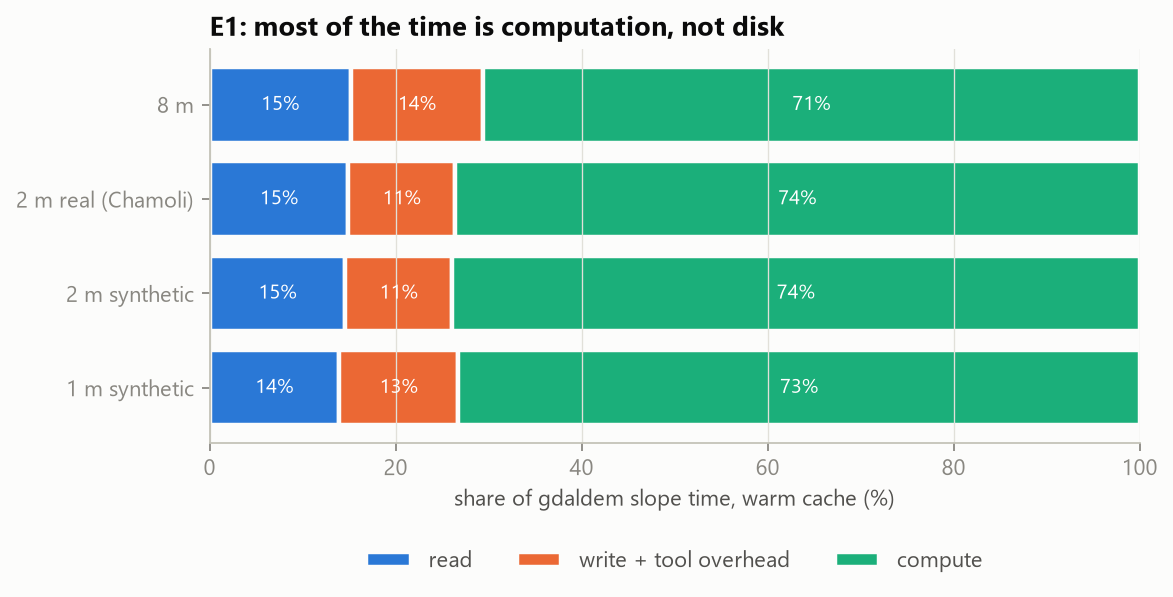
\includegraphics[width=0.49\linewidth]{e1_stages.png}\hfill
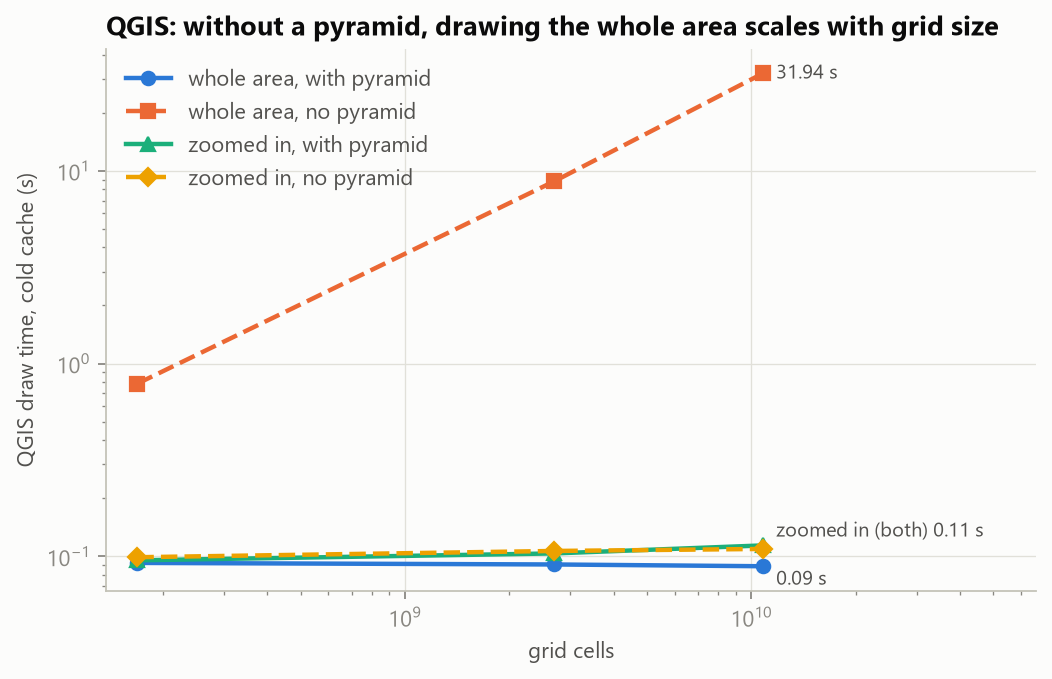
\includegraphics[width=0.46\linewidth]{e1q_render.png}
\caption{Left: share of \texttt{gdaldem}'s slope time per stage; computation is about 73\% at every size. Right:
QGIS draw time. Without a pyramid a whole-area redraw reads the full-resolution grid and grows with its size; with
the pyramid, and for zoomed-in views, the cost stays constant.}
\label{fig:qgis}
\end{figure}

Opening a layer takes 0.02--0.03\,s in every case. Only zoomed-out views need the pyramid: a zoomed-in view reads
just its window and stays at about 0.1\,s even without one. Without a pyramid, every whole-area redraw of the 1\,m
grid reads its whole full-resolution level, about 12.7\,GB, which is 360$\times$ slower than with the pyramid and
close to the 29\,s that a pure read and decompress of it takes.

\subsection{Answer to Q1}
On a 16\,GB laptop with an NVMe SSD, the standard tools \emph{do not stop working} at 1\,m; they stop being
\emph{practical}:
\begin{itemize}
  \item \textbf{processing} is limited by \textbf{single-threaded computation}: 3.5\,min for one slope pass at 1\,m,
  using 1 of 22 threads, with the disk and memory far from their limits;
  \item \textbf{display} is limited by \textbf{reading full-resolution data}: without a pyramid a whole-area redraw
  grows with the grid (32\,s at 1\,m); with one it stays at 0.09\,s.
\end{itemize}
This differs from the pilot of the literature review, which saw caching triple the run time at 5\,m. With a verified
cold cache and a fast NVMe SSD the cache state changes run time by at most 2\%. The pilot timed runs through the
QGIS interface on a different laptop, so its first runs probably included one-off start-up and loading costs.

%=====================================================================
\section{Our terrain engine on the CPU and the GPU (E3, E4)}\label{sec:engine}
E1 shows that the largest gain should come from parallel computation. Reading and writing take about 27\% of each
\texttt{gdaldem} run, so by Amdahl's law parallel computation alone can make it at most about 3.7$\times$ faster
(the whole run speeds up at most $1/(1-p)$ when a share $p$ becomes infinitely fast). We built our own engine to
remove the computation bottleneck and to find where it moves next.

\subsection{Design}
\paragraph{CPU pipeline.} The grid is processed in $2048\times2048$-cell windows, each read with a one-cell border
(halo), so that the $3\times3$ operators are exact at window edges. Three stages overlap: four reader threads (each
with its own GDAL handle; at most six windows in flight, so memory stays bounded), the compute kernel in the main
thread, and one writer thread, since GDAL's multi-threading documentation advises against writing from several
threads. The kernel is compiled with Numba \cite{numba} and spread over all cores. Slope, aspect and hillshade can be
computed in one fused pass, since they share the same gradient.

\paragraph{GPU.} The same pipeline with only the compute stage replaced. Each window is copied into a pinned
(page-locked) host buffer, copied to the GPU, processed by our own CUDA kernels (compiled at run time through CuPy
\cite{cupy}; one GPU thread per cell; three products fused), and copied back. Windows alternate between two CUDA
streams, so that the copies of one window overlap the kernel of the next. Arithmetic is float32: GDAL itself adds
the Horn neighbour values in float32, and laptop GPUs run float64 at 1/64 of the float32 rate. For safety, GPU
memory was capped at 4\,GiB, and the harness waited before every run until the GPU was below 75\,$^\circ$C (it would
have stopped at 85\,$^\circ$C). The GPU reached at most 63\,$^\circ$C and used at most 2.0\,GiB.

\paragraph{Correctness.} The engine implements all ten \texttt{gdaldem} configurations with \texttt{gdaldem}'s
conventions (nodata border, flat-cell aspect, hillshade scaling). Unit tests (119 at this stage) compare every
kernel with \texttt{gdaldem} on two $1024^2$ crops. A full-grid check compares both engines with \texttt{gdaldem} on
every cell of the whole 90\,m, 30\,m, 8\,m and 2\,m real grids for all ten configurations (1.3\,M to 247\,M valid
cells per grid). The GPU engine has identical nodata masks and no cell beyond tolerance in any configuration. The
float64 CPU engine differs only in Horn aspect on a few nearly flat cells (at most 0.08\% of cells) and in Horn slope
on one cell (0.022$^\circ$ against a 0.02$^\circ$ tolerance), because \texttt{gdaldem} adds the Horn neighbours in
float32. With that rounding reproduced, every cell of all four grids matches.

\subsection{CPU engine (E3): speed and memory}
\begin{table}[!htbp]
\centering\small
\caption{Slope (Horn), engine against \texttt{gdaldem}, warm cache. ``Same cores'': the engine pinned to the 12
performance-core threads that \texttt{gdaldem} used.}
\label{tab:e3}
\begin{tabularx}{\linewidth}{lrRRRRR}
\toprule
Grid & Cells & \texttt{gdaldem} & Engine, same cores & Speed-up & Engine, 22 threads & Engine peak memory \\
\midrule
8\,m & 169\,M & 4.02\,s & 1.94\,s & 2.1$\times$ & 2.28\,s & 1.35\,GB \\
2\,m real & 264\,M & 6.63\,s & 2.53\,s & 2.6$\times$ & 2.72\,s & 1.37\,GB \\
2\,m synthetic & 2.7\,B & 53.7\,s & 16.3\,s & 3.3$\times$ & 16.4\,s & 1.42\,GB \\
1\,m synthetic & 10.8\,B & 208.4\,s & \textbf{60.3\,s} & \textbf{3.5$\times$} & 68.2\,s & 1.43\,GB \\
\bottomrule
\end{tabularx}
\end{table}

\begin{figure}[!htbp]
\centering
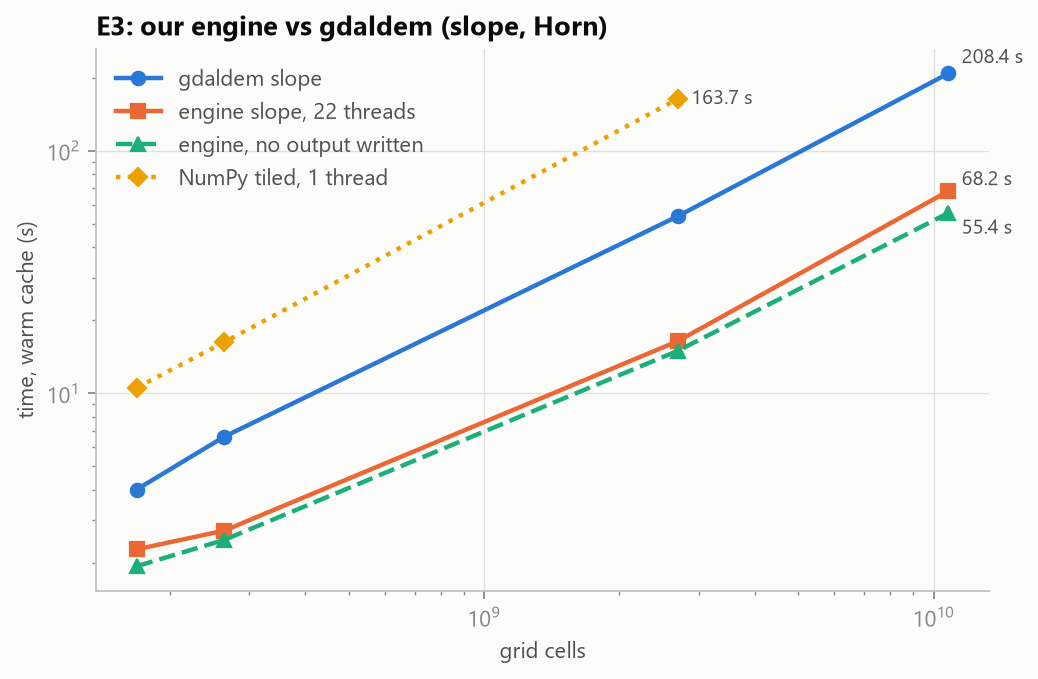
\includegraphics[width=0.49\linewidth]{e3_scaling.png}\hfill
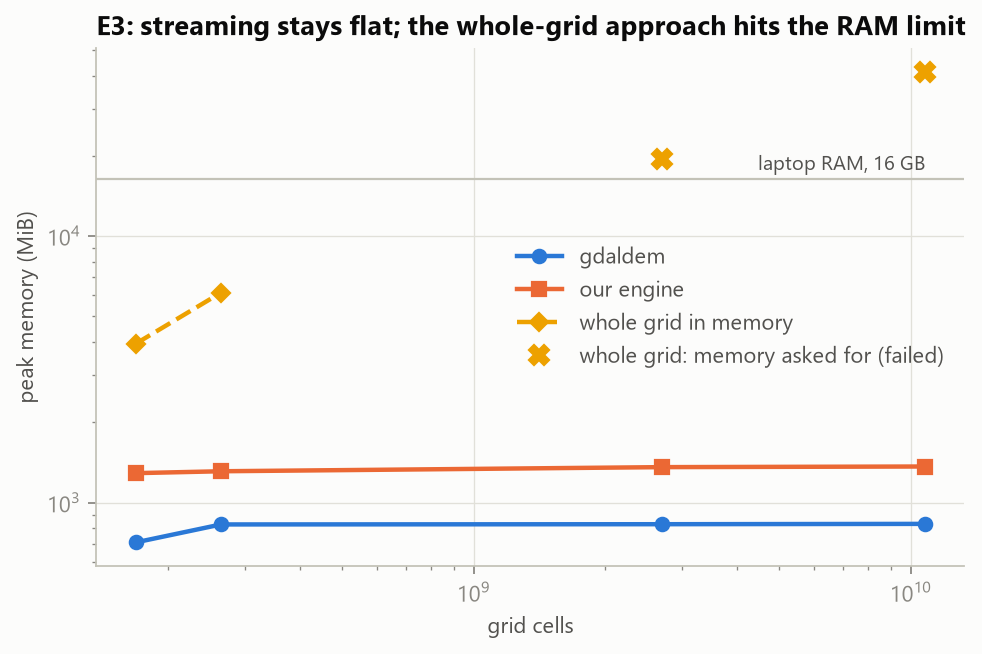
\includegraphics[width=0.49\linewidth]{e3_memory.png}
\caption{E3. Left: slope run time against grid size. Right: peak memory. The engine stays flat at about 1.4\,GB;
the whole-grid NumPy program needs about 24 bytes per cell and fails on the 2\,m synthetic and 1\,m grids.}
\label{fig:e3}
\end{figure}

\begin{itemize}
  \item \textbf{2.1--3.5$\times$ faster on the same cores, growing with size} (Table~\ref{tab:e3}). At 1\,m the
  engine needs about 5.6\,ns per cell against \texttt{gdaldem}'s 19\,ns. Small grids gain less, because about 1\,s
  of every run is fixed cost (Python start-up and loading the compiled kernel).
  \item \textbf{12 performance-core threads beat all 22} (1\,m: 60\,s against 68\,s): the work is split evenly, so
  the slower efficiency and low-power cores hold the other threads up.
  \item \textbf{Memory is flat} at about 1.4\,GB for every size (Figure~\ref{fig:e3}).
  \item \textbf{Where the simple approach breaks.} A naive program that loads the whole grid into NumPy needs about
  24 bytes per cell (4.1\,GB at 8\,m, 6.4\,GB at 2\,m real). On the 2\,m synthetic grid it held 9.6\,GB when a
  further 10.7\,GB allocation was refused (the whole run would need about 65\,GB); at 1\,m its first allocation of
  43\,GB was refused. On this laptop whole-grid processing stops working at roughly 0.5--0.7 billion cells;
  streaming tools (\texttt{gdaldem}, our engine) have no such limit.
  \item \textbf{The speed comes from the compiled parallel kernel, not from tiling alone}: the same pipeline with a
  single-threaded NumPy kernel is 2.6--3$\times$ \emph{slower} than \texttt{gdaldem}.
  \item \textbf{Every operator is faster}: all ten configurations run 1.3--2.0$\times$ faster at 8\,m and
  1.7--2.6$\times$ faster on the 2\,m real grid. On these grids the engine takes the same time for every operator,
  because fixed start-up and I/O dominate, not the arithmetic.
\end{itemize}

\begin{table}[!htbp]
\centering\small
\caption{Slope + aspect + hillshade, warm cache. \texttt{gdaldem} was not run for aspect on the synthetic grids, so
there only slope + hillshade can be compared (a lower bound for the gain).}
\label{tab:fused}
\begin{tabularx}{\linewidth}{lRRRRR}
\toprule
Grid & \texttt{gdaldem}, 3 runs & CPU engine, 3 runs & CPU engine, fused & GPU engine, fused & Fused CPU vs \texttt{gdaldem} \\
\midrule
8\,m & 11.3\,s & 6.6\,s & 3.3\,s & \textbf{2.56\,s} & 3.4$\times$ \\
2\,m real & 18.5\,s & 7.9\,s & 4.4\,s & \textbf{3.13\,s} & 4.2$\times$ \\
2\,m synthetic & ($>$94.7\,s) & 49.0\,s & 34.4\,s & \textbf{21.0\,s} & $\geq$2.8$\times$ \\
1\,m synthetic & ($>$367\,s) & -- & 134.8\,s & \textbf{81.4\,s} & $\geq$2.7$\times$ \\
\bottomrule
\end{tabularx}
\end{table}

\paragraph{Three products in one pass} cost little more than one (Table~\ref{tab:fused}): the fused pass reads the
input once and computes the gradient once. At 1\,m it writes 97\,GB, and its writer is busy for 121\,s of the
135\,s, so it is write-bound.

\subsection{CPU engine: where the time goes}
\begin{table}[!htbp]
\centering\small
\caption{CPU engine, slope, all 22 threads, warm cache. ``Wait'' columns: time the compute thread sat idle. The
writer works in parallel; ``writer busy'' is its own working time.}
\label{tab:stages3}
\begin{tabularx}{\linewidth}{lRRRRRRR}
\toprule
Grid & Total & Start-up & Wait for input & Compute & Wait for writer & Writer busy & Written \\
\midrule
8\,m & 2.28\,s & 0.52\,s & 0.27\,s & 0.98\,s & 0.25\,s & 1.01\,s & 0.71\,GB \\
2\,m real & 2.72\,s & 0.50\,s & 0.39\,s & 1.24\,s & 0.30\,s & 1.48\,s & 1.10\,GB \\
2\,m synthetic & 16.4\,s & 0.63\,s & 3.4\,s & 8.9\,s & 3.3\,s & 14.6\,s & 10.9\,GB \\
1\,m synthetic & 68.2\,s & 0.62\,s & 9.3\,s & 33.1\,s & 24.8\,s & \textbf{65.3\,s} & 43.4\,GB \\
1\,m, no output & 55.4\,s & 0.60\,s & \textbf{22.9\,s} & 31.4\,s & 0 & 0 & 0 \\
\bottomrule
\end{tabularx}
\end{table}

\begin{itemize}
  \item \textbf{The run is now limited by moving data} (Table~\ref{tab:stages3}). At 1\,m the kernel needs 33\,s,
  while the single writer thread is busy for 65\,s writing 43\,GB (about 0.66\,GB/s): the run is
  \emph{write-bound}. Without output it is \emph{read-bound}: 23\,s of waiting for windows to be decompressed.
  \item \textbf{Reading is limited by decompression, not by the disk.} With no output, 8 reader threads instead of 4
  cut the read wait on the 2\,m synthetic grid from 5.8\,s to 1.2\,s; with output written the change gives nothing,
  because the writer is then the limit. Cold and warm cache give almost the same time (1\,m: 67\,s and 68\,s).
  \item \textbf{Compressed output} (ZSTD level 1) is 40\% smaller (2\,m synthetic: 6.6\,GB instead of 10.9\,GB) but
  slower (21.2\,s against 16.4\,s), because compression takes CPU time away from the kernel.
  \item \textbf{More threads stop helping early.} Inside the pipeline the kernel speeds up only 2.2--2.8$\times$
  from 1 to 22 threads; alone, in memory, it scales to about 16 threads (9.5\,ns per cell with 1 thread, 1.7\,ns
  with 16). In the pipeline it shares the cores with decompression and writing.
  \item \textbf{The halo makes small windows slow.} The input is stored in compressed $512\times512$ tiles, and a
  window's one-cell border forces the neighbouring tiles to be decompressed again: $(w/512+2)^2$ tiles instead of
  $(w/512)^2$ for a window of $w$ cells per side, 9$\times$ the work at $w=512$ and 2.25$\times$ at 2048. A 512 window
  is up to 2.2$\times$ slower; an 8192 window holds 7.4\,GB in flight for no gain. 2048 is the best size overall.
\end{itemize}

\subsection{GPU engine (E4)}
\begin{table}[!htbp]
\centering\small
\caption{Slope (Horn), warm cache: \texttt{gdaldem}, CPU engine (12 threads) and GPU engine.}
\label{tab:e4}
\begin{tabularx}{\linewidth}{lRRRRRR}
\toprule
Grid & \texttt{gdaldem} & CPU engine & GPU engine & GPU vs CPU & GPU vs \texttt{gdaldem} & GPU, no output \\
\midrule
8\,m & 4.02\,s & 1.94\,s & 1.90\,s & 1.0$\times$ & 2.1$\times$ & 1.80\,s \\
2\,m real & 6.63\,s & 2.53\,s & 2.18\,s & 1.2$\times$ & 3.0$\times$ & 2.03\,s \\
2\,m synthetic & 53.7\,s & 16.3\,s & \textbf{11.3\,s} & 1.4$\times$ & 4.7$\times$ & 9.3\,s \\
1\,m synthetic & 208.4\,s & 60.3\,s & \textbf{43.8\,s} & 1.4$\times$ & \textbf{4.75$\times$} & 33.9\,s \\
\bottomrule
\end{tabularx}
\end{table}

\begin{table}[!htbp]
\centering\small
\caption{Crossover test: one slope window held in memory, no disk (ms per window, median). The GPU times
include the copies to and from the GPU unless stated.}
\label{tab:crossover}
\begin{tabularx}{\linewidth}{lRRRRR}
\toprule
Window & CPU kernel, 12 threads & GPU incl.\ copies (pinned) & GPU kernel only & GPU vs CPU & Copies' share of GPU time \\
\midrule
$128^2$ & \textbf{0.04} & 0.17 & 0.04 & 0.24$\times$ & 74\% \\
$256^2$ & \textbf{0.20} & 0.33 & 0.05 & 0.59$\times$ & 86\% \\
$512^2$ & 0.54 & \textbf{0.41} & 0.05 & 1.3$\times$ & 88\% \\
$1024^2$ & 2.13 & \textbf{0.98} & 0.07 & 2.2$\times$ & 93\% \\
$2048^2$ & 9.38 & \textbf{3.85} & 0.18 & 2.4$\times$ & 95\% \\
$8192^2$ & 140.1 & \textbf{61.7} & 2.62 & 2.3$\times$ & 96\% \\
\bottomrule
\end{tabularx}
\end{table}

\begin{itemize}
  \item \textbf{The GPU computes 50$\times$ faster, but the run is only 1.0--1.4$\times$ faster}
  (Table~\ref{tab:e4}). The GPU kernel needs 1.1\,s for the whole 10.8-billion-cell grid, where the CPU engine's
  kernel needed 34\,s.
  \item \textbf{Copying is 95\% of the GPU's own time} (Table~\ref{tab:crossover}). For a $2048^2$ window the kernel
  takes 0.18\,ms and kernel plus copies 3.85\,ms. Over PCIe 4.0 $\times$8 a cell costs about 0.9\,ns to move in and
  out, against 0.04\,ns to compute.
  \item \textbf{The GPU only pays off above a minimum size}: from $512^2$ cells for slope and from $256^2$ for three
  products. Below that a GPU round trip, at least about 0.17\,ms, is slower than the CPU kernel.
  \item \textbf{Three products gain the most}: a fused pass takes 81\,s at 1\,m against 135\,s on the CPU
  (1.7$\times$), and 3.1\,s on the 2\,m real grid against 18.5\,s for three \texttt{gdaldem} runs (5.9$\times$).
  \item \textbf{GPU memory is never the limit}: window by window the engine uses at most 2.0\,GiB of the 8\,GiB.
  Sending a whole grid at once would need 22\,GB at 2\,m synthetic and 86\,GB at 1\,m. As on the CPU, only tiling
  scales.
\end{itemize}

\begin{figure}[!htbp]
\centering
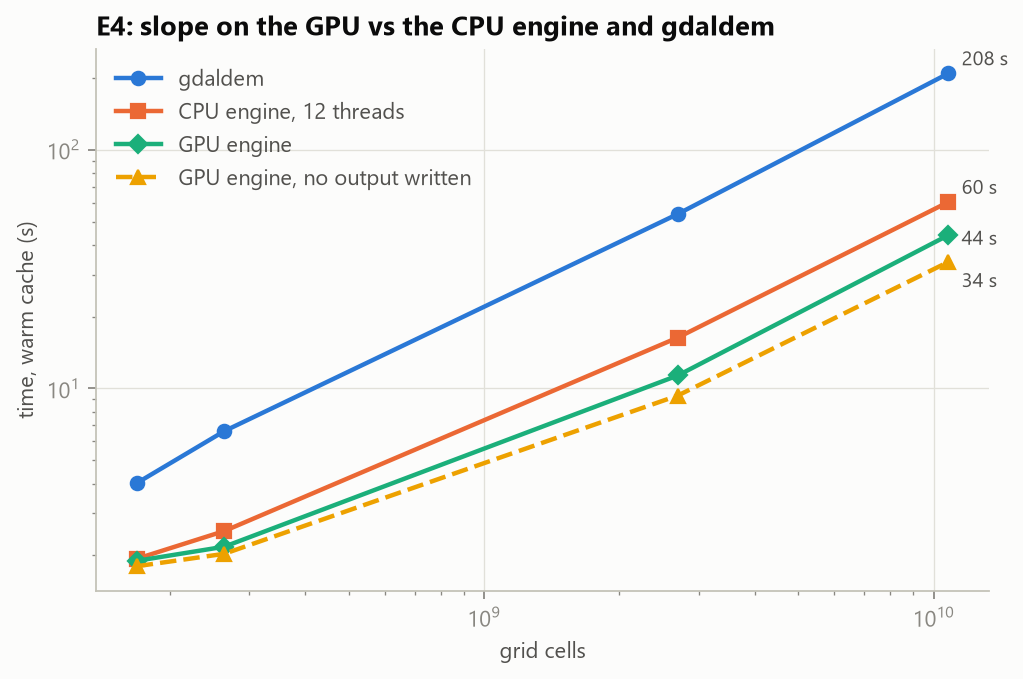
\includegraphics[width=0.49\linewidth]{e4_scaling.png}\hfill
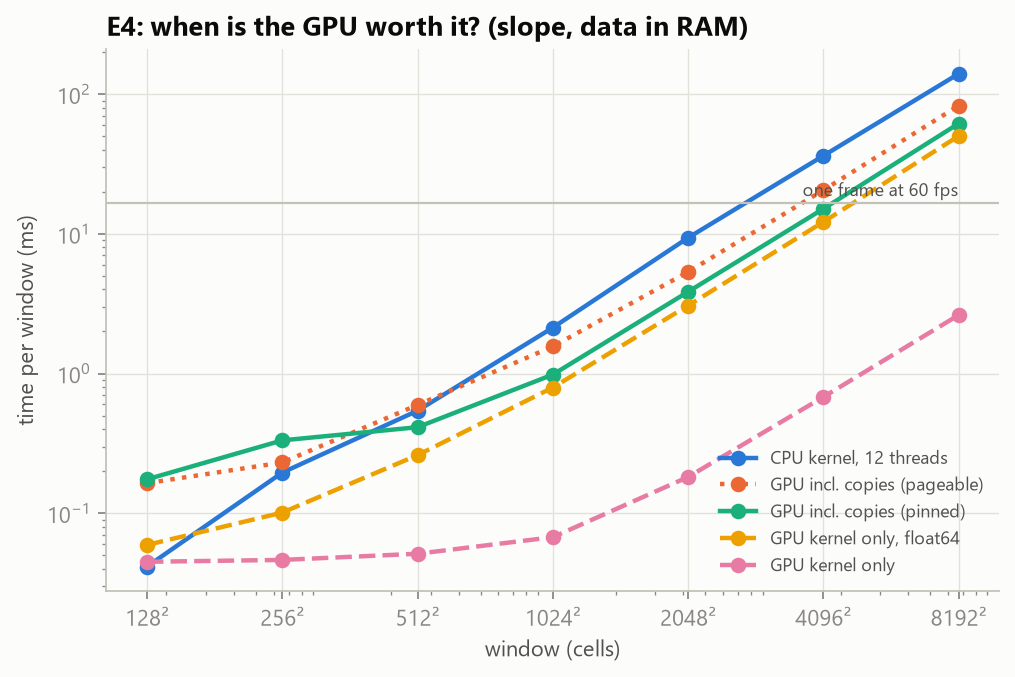
\includegraphics[width=0.49\linewidth]{e4_crossover.png}
\caption{E4. Left: slope run time against grid size for \texttt{gdaldem}, the CPU engine and the GPU engine.
Right: one window held in memory. The GPU kernel alone is about 50$\times$ faster than the 12-thread CPU kernel;
with the copies it is only 2.2--2.4$\times$ faster, and below about $512^2$ cells it is slower than the CPU.}
\label{fig:e4}
\end{figure}

\paragraph{How the GPU is used matters more than the GPU.} On the 2\,m synthetic grid a straightforward port (the
NumPy code run on CuPy arrays, float64, a temporary array for every intermediate result) takes 17.0\,s, slower than
the CPU engine (16.3\,s). Our own CUDA kernel brings the run to 12.6\,s and pinned buffers to 11.1\,s. Each step
roughly halves the GPU stage (14.5 $\rightarrow$ 7.6 $\rightarrow$ 3.7 $\rightarrow$ 2.0\,s with two streams), but the
total stops improving once reading and writing dominate. float64 arithmetic makes the kernel 8--24$\times$ slower and
leaves the total almost unchanged (11.5\,s against 11.3\,s).

\paragraph{The bottleneck moves.} At 1\,m the GPU engine's main thread spends 25.7\,s waiting for input to be
decompressed and only 7.8\,s on the GPU. With 8 reader threads instead of 4 the read wait falls to 3.2\,s, but the
writer then becomes the limit (it waits 30.6\,s for 43\,GB to be written at about 1.1\,GB/s), and the total only
goes from 43.8\,s to 42.6\,s. Each fix exposes the next stage: \emph{computation $\rightarrow$ decompression
$\rightarrow$ writing} (Figure~\ref{fig:stages}).

\begin{figure}[!htbp]
\centering
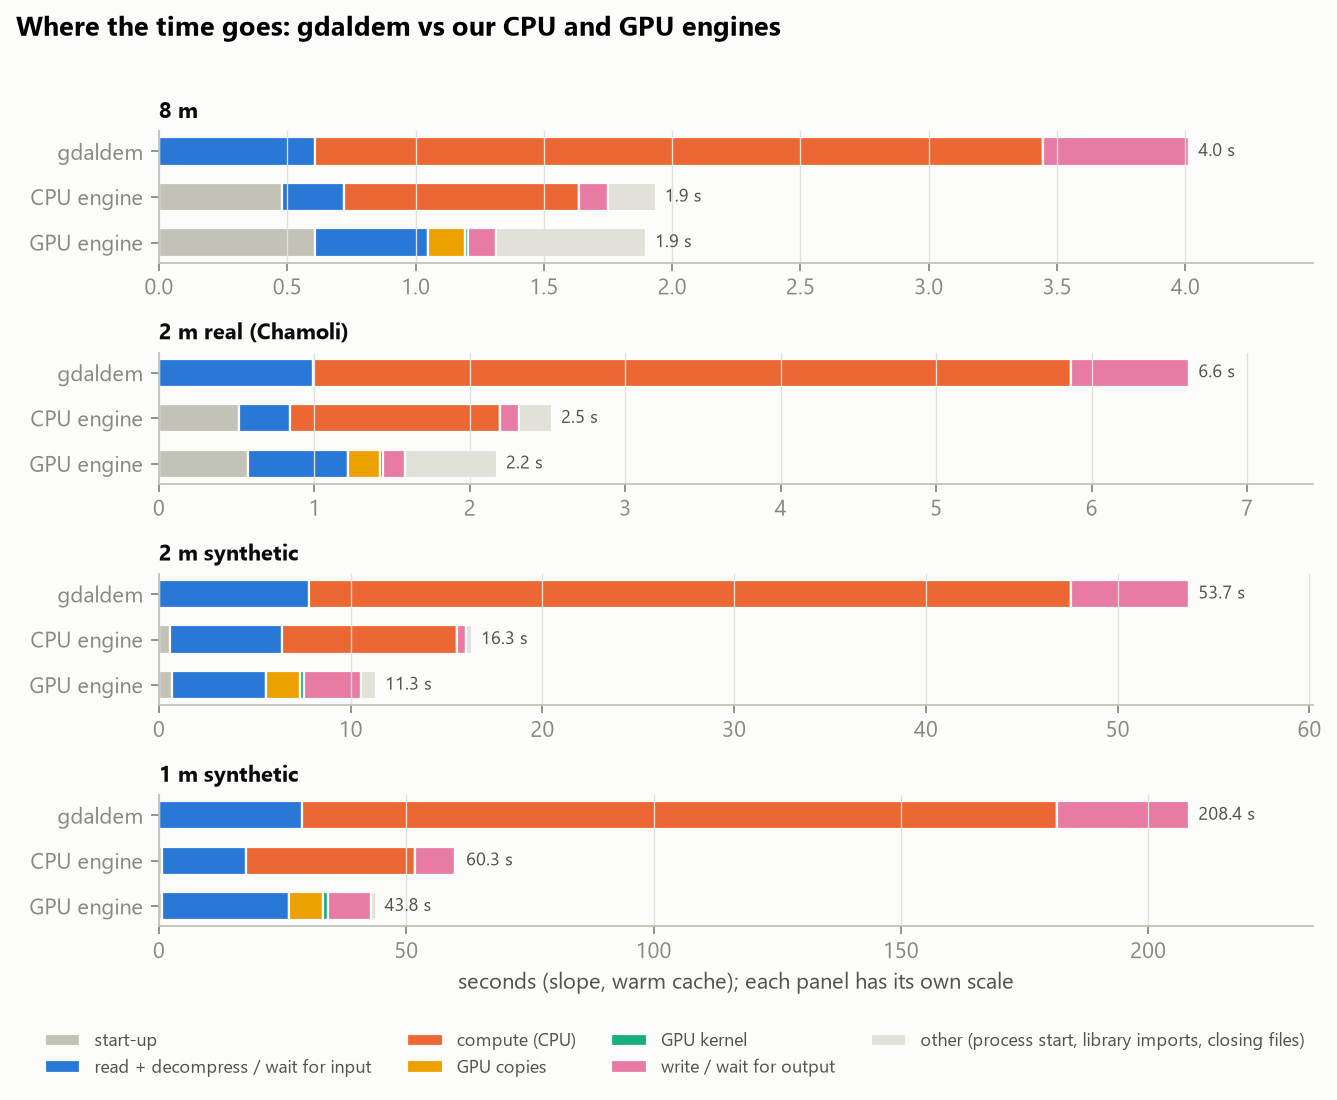
\includegraphics[width=0.74\linewidth]{e4_stages.png}
\caption{Where the time goes (slope, warm). \texttt{gdaldem}: stages from the stage split, one after the other.
Engines: how the main thread spends the run (the writer works in parallel, so only waiting for it appears). From
\texttt{gdaldem} to the CPU engine to the GPU engine, computation shrinks and reading, copying and writing remain.}
\label{fig:stages}
\end{figure}

\subsection{Answer to Q2}
\texttt{gdaldem} is limited by single-threaded computation. Our parallel CPU engine removes most of it and becomes
limited by decompressing the input and writing the output. The GPU removes computation almost entirely (1.1\,s for
10.8 billion cells), and what remains is reading, writing and copying over PCIe. A GPU is worth adding where
computation is still a large share: several products at once, heavier operators, or results that are not written to
disk. For on-demand display, computation is cheap on both devices: a $512^2$ tile takes 0.5\,ms (slope) or 1.3\,ms
(three products) on the CPU and 0.4--0.5\,ms on the GPU including copies. The time per view is then set by reading
and decoding elevation data, which is what the pyramid and a cache of decoded data address.

%=====================================================================
\section{Derivatives on demand from the pyramid (E5)}\label{sec:pyramid}
A viewer showing a large area cannot use the full-resolution DEM. It reads a coarser pyramid level and computes slope
there. E5 measures how far that slope is from what a full-resolution computation would show for the same screen
cell, and how much time it saves (gap G2).

\subsection{Method}
Accuracy needs real data, so E5 uses only the two real high-resolution DEMs: Chamoli 2\,m (15120 $\times$ 17460
cells, pyramid levels 1--6 at 4 to 128\,m; the main result) and the HMA 8\,m tile (13140 $\times$ 12825 cells,
levels 1--5 at 16 to 256\,m), each with its own COG overviews.
\begin{itemize}
  \item \textbf{On demand:} slope (Horn) and aspect computed by our engine's kernel on the level-$k$ DEM, with that
  level's cell size.
  \item \textbf{Truth:} slope and aspect computed at full resolution, then averaged over exactly the fine cells each
  coarse cell covers (slope: mean; aspect: circular mean of the fine directions). This is what a screen pixel of that
  size \emph{should} show: the average steepness of the ground under it.
  \item \textbf{Footprints.} GDAL halves each level's size and rounds down, so when the grid size is not divisible by
  $2^k$, a level cell is slightly larger than $2^k$ fine cells (on Chamoli, level 3 cells cover 8.002 fine rows
  instead of 8). Each coarse cell's footprint is therefore taken from its geometry (the fine cells whose centres fall
  inside it), and every measurement was repeated on an exact power-of-two pyramid built by ourselves.
  \item \textbf{Scored cells:} only cells whose footprint and 8 neighbours contain no nodata at full resolution, so
  data gaps never enter the comparison: 61 million down to 51 thousand cells per level on Chamoli. Aspect is scored
  where the true slope is at least 5$^\circ$ and the fine directions agree (mean resultant length $\geq0.5$), which
  keeps 87--99\% of the scored slope cells.
  \item \textbf{Time:} three ways to serve a view at level $k$, measured in one long-running process on the 12
  performance-core threads: \emph{on demand} (read the view from level $k$ plus a one-cell halo and compute),
  \emph{full resolution} (read the same ground at full resolution, compute, average to level $k$: the exact answer
  without precomputation), and \emph{precomputed} (read the view from a slope pyramid built in advance). Views are one
  $512\times512$ display tile at 8 random places per level (each at least 90\% valid) and the whole grid. A fresh
  dataset handle is opened for every measurement, so GDAL's block cache never hides the decoding.
\end{itemize}

\subsection{Slope error per pyramid level}
\begin{table}[!htbp]
\centering\small
\caption{Slope computed on demand from each pyramid level against the full-resolution truth. Last column: the same
with an exact power-of-two pyramid instead of GDAL's overviews.}
\label{tab:err}
\begin{tabularx}{\linewidth}{llRRRRRRR}
\toprule
DEM & Level & Cells scored & RMSE & Bias & $>$5$^\circ$ & $>$10$^\circ$ & Shown / true mean & RMSE exact \\
\midrule
Chamoli 2\,m & 4\,m & 61.4\,M & \textbf{2.3$^\circ$} & $-$0.5$^\circ$ & 4.1\% & 0.7\% & 0.99 & 2.3$^\circ$ \\
 & 8\,m & 15.2\,M & \textbf{4.4$^\circ$} & $-$1.2$^\circ$ & 15.5\% & 4.1\% & 0.97 & 4.4$^\circ$ \\
 & 16\,m & 3.7\,M & \textbf{5.6$^\circ$} & $-$2.2$^\circ$ & 23.4\% & 7.2\% & 0.94 & 5.6$^\circ$ \\
 & 32\,m & 0.91\,M & \textbf{6.4$^\circ$} & $-$3.3$^\circ$ & 30.5\% & 10.3\% & 0.91 & 6.4$^\circ$ \\
 & 64\,m & 0.22\,M & \textbf{7.9$^\circ$} & $-$5.0$^\circ$ & 43.1\% & 17.1\% & 0.87 & 7.8$^\circ$ \\
 & 128\,m & 51\,k & \textbf{10.0$^\circ$} & $-$7.3$^\circ$ & 57.8\% & 28.2\% & 0.81 & 9.9$^\circ$ \\
\midrule
HMA 8\,m & 16\,m & 29.6\,M & \textbf{2.6$^\circ$} & $-$0.7$^\circ$ & 6.6\% & 0.9\% & 0.98 & 2.4$^\circ$ \\
 & 32\,m & 6.5\,M & \textbf{4.0$^\circ$} & $-$1.6$^\circ$ & 15.6\% & 3.0\% & 0.95 & 3.9$^\circ$ \\
 & 64\,m & 1.3\,M & \textbf{5.3$^\circ$} & $-$2.9$^\circ$ & 26.3\% & 6.9\% & 0.90 & 5.3$^\circ$ \\
 & 128\,m & 0.23\,M & \textbf{6.9$^\circ$} & $-$4.5$^\circ$ & 40.5\% & 13.3\% & 0.83 & 6.9$^\circ$ \\
 & 256\,m & 29\,k & \textbf{9.0$^\circ$} & $-$6.8$^\circ$ & 58.7\% & 24.9\% & 0.73 & 8.8$^\circ$ \\
\bottomrule
\end{tabularx}
\end{table}

\begin{figure}[!htbp]
\centering
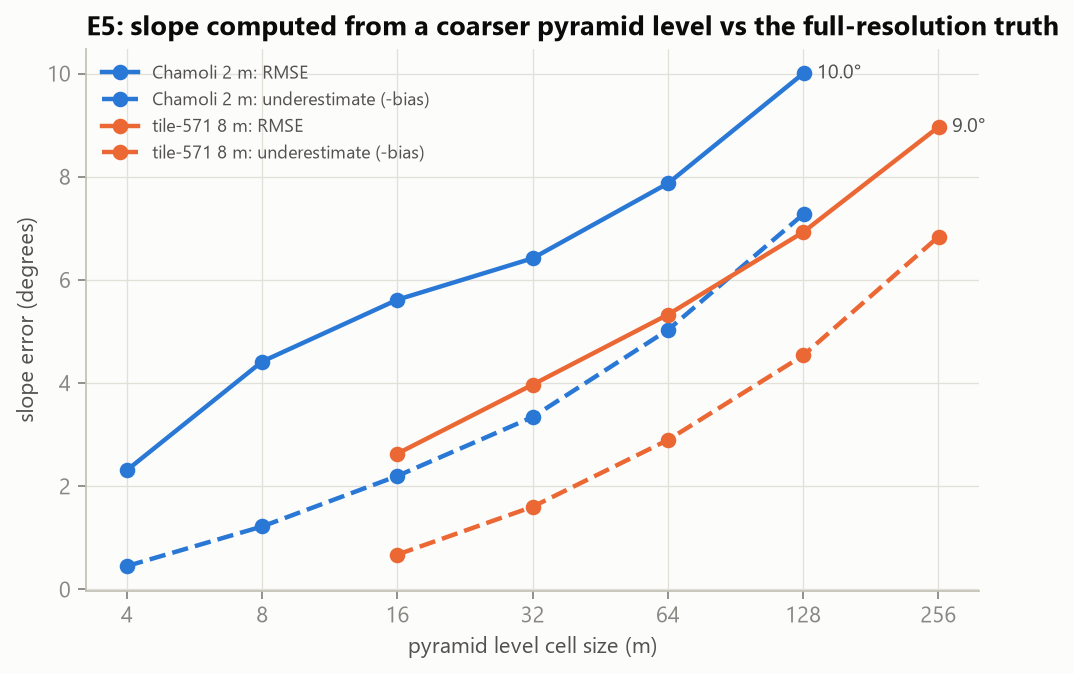
\includegraphics[width=0.49\linewidth]{e5_error_by_level.png}\hfill
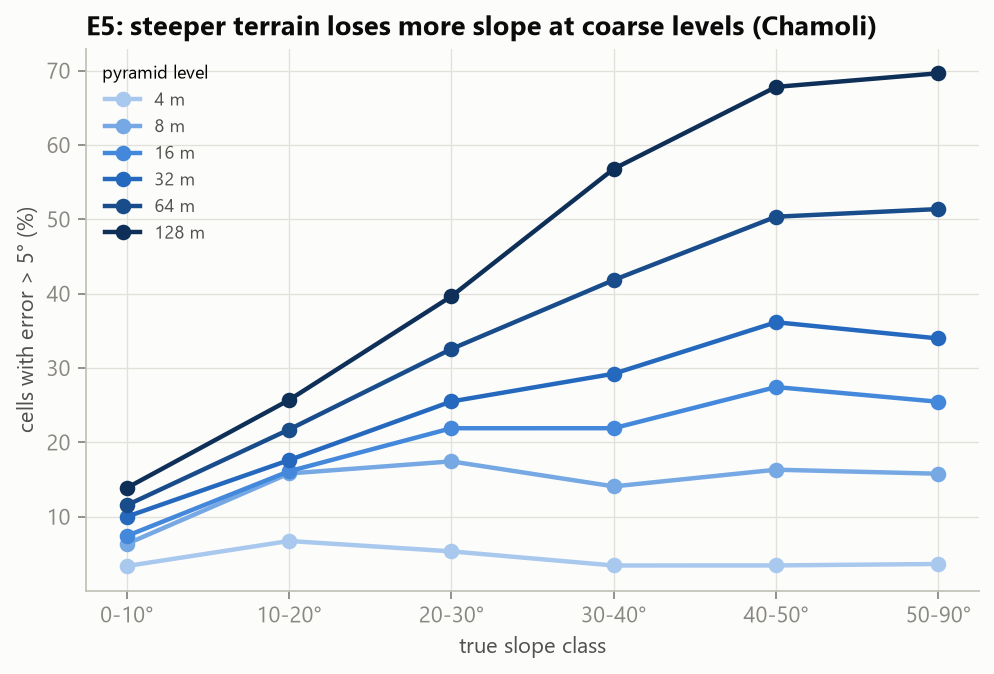
\includegraphics[width=0.49\linewidth]{e5_by_class.png}
\caption{E5. Left: slope RMSE and underestimate ($-$bias) per pyramid level for both DEMs. Right: share of cells
off by more than 5$^\circ$ by true-slope class (Chamoli): steep terrain loses the most.}
\label{fig:e5err}
\end{figure}

\begin{itemize}
  \item \textbf{Slope from a coarse level is too low, and more so the coarser the level} (Table~\ref{tab:err},
  Figure~\ref{fig:e5err}). Averaging the DEM smooths the terrain before slope is computed, which removes steepness:
  the mean slope shown drops from 99\% to 81\% of the true mean on Chamoli. This agrees with the long-known decrease
  of computed slope with grid size \cite{zhang}; what is new is the measurement on pyramid levels, together with the
  time saved.
  \item \textbf{What matters is how many levels up, not the cell size in metres.} The two DEMs give similar errors
  for the same number of levels up (within 0.5$^\circ$ up to four levels): about 2.5$^\circ$ RMSE one level up, then
  on average about 1.5$^\circ$ more per further level (single steps 0.8--2.1$^\circ$).
  \item \textbf{GDAL's overviews behave like an exact pyramid}: within 0.2$^\circ$ RMSE at every level, although
  their cells are not exactly $2^k$ fine cells. A viewer can use COG overviews as they are.
\end{itemize}

\begin{figure}[!htbp]
\centering
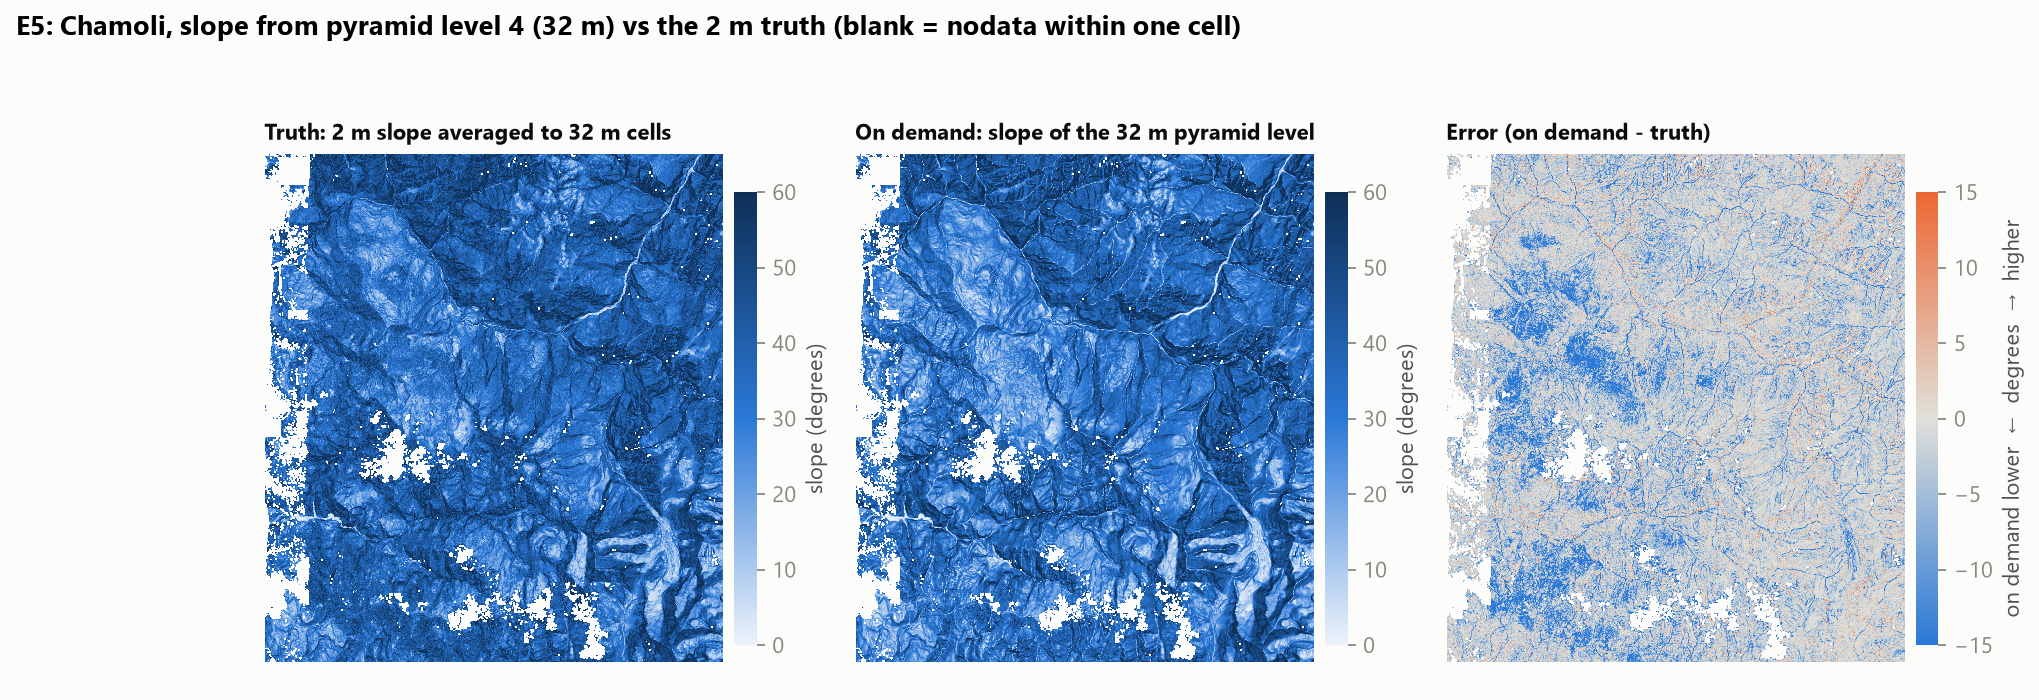
\includegraphics[width=\linewidth]{e5_maps.png}
\caption{Chamoli at 32\,m. Left: truth (2\,m slope averaged to 32\,m cells). Middle: slope computed on demand from
the 32\,m pyramid level. Right: error; blue means the on-demand slope is lower. The on-demand map keeps every valley,
ridge and landslide scar but is lower almost everywhere, most on rough, broken slopes.}
\label{fig:maps}
\end{figure}

\subsection{Steep terrain, thresholds and aspect}
\begin{table}[!htbp]
\centering\small
\caption{Chamoli: slope bias ($^\circ$) by true-slope class, and the share of cells at or above 45$^\circ$ in truth
and on demand.}
\label{tab:class}
\begin{tabularx}{\linewidth}{lRRRRRRRR}
\toprule
Level & 0--10$^\circ$ & 10--20$^\circ$ & 20--30$^\circ$ & 30--40$^\circ$ & 40--50$^\circ$ & 50--90$^\circ$ &
$\geq$45$^\circ$ truth & $\geq$45$^\circ$ shown \\
\midrule
4\,m & $-$0.1 & $-$0.2 & $-$0.3 & $-$0.3 & $-$0.6 & $-$0.8 & 33.2\% & 32.1\% \\
8\,m & $-$0.0 & $-$0.2 & $-$0.7 & $-$1.0 & $-$1.6 & $-$2.0 & 32.3\% & 29.2\% \\
16\,m & $-$0.5 & $-$0.8 & $-$1.4 & $-$2.0 & $-$2.8 & $-$3.0 & 30.8\% & 25.7\% \\
32\,m & $-$0.9 & $-$1.5 & $-$2.6 & $-$3.3 & $-$4.0 & $-$3.9 & 29.3\% & 21.9\% \\
64\,m & $-$0.7 & $-$1.9 & $-$3.5 & $-$5.1 & $-$6.0 & $-$5.9 & 28.4\% & 16.5\% \\
128\,m & $-$0.8 & $-$2.4 & $-$4.3 & $-$7.3 & $-$8.8 & $-$8.9 & 27.4\% & \textbf{10.1\%} \\
\bottomrule
\end{tabularx}
\end{table}

\begin{itemize}
  \item \textbf{Steep cells lose the most} (Table~\ref{tab:class}). At 32\,m the bias is $-0.9^\circ$ on
  0--10$^\circ$ ground but $-4.0^\circ$ on 40--50$^\circ$ ground, and 36\% of the 40--50$^\circ$ cells are off by more
  than 5$^\circ$, against 10\% on flat ground (at 128\,m: 68\% against 14\%). The map in Figure~\ref{fig:maps} shows
  the same pattern.
  \item \textbf{Slope thresholds shift.} Many uses of slope are a threshold, such as landslide susceptibility or
  ``too steep to build''. One level up, a threshold map at 30$^\circ$ or 45$^\circ$ is still 97\% the same. Four
  levels up, a quarter of the terrain at or above 45$^\circ$ has disappeared (29.3\% $\rightarrow$ 21.9\%), and six
  levels up almost two thirds (27.4\% $\rightarrow$ 10.1\%). For display this is acceptable; for analysis that uses
  thresholds it is not.
  \item \textbf{Aspect survives coarse levels much better.} The direction a slope faces is set by large landforms.
  On Chamoli the median aspect error is 1.8$^\circ$ at 4\,m, 3.8$^\circ$ at 8\,m, 6.3$^\circ$ at 32\,m and
  8.5$^\circ$ at 128\,m; only 1.4\% (4\,m) to 13.7\% (128\,m) of cells are off by more than 22.5$^\circ$, the width of
  one 16-point compass sector. The 8\,m DEM gives the same picture (median 2.8$^\circ$ at 16\,m to 9.9$^\circ$ at
  256\,m).
\end{itemize}

\paragraph{Pyramid error against differences between data sources.} Over the Chamoli footprint, against the same
truth, the 2\,m data averaged to a coarser size (a pyramid level) is always closer to the truth than an independent
DEM measured at that size by another sensor (Table~\ref{tab:sensors}). At 8\,m the difference between the two
sources is larger than what the pyramid loses; at 90\,m the sources agree well, and most of the error of both is
simply the coarse resolution. When a high-resolution DEM exists, its pyramid is the better coarse product.

\begin{table}[!htbp]
\centering\small
\caption{Slope RMSE against the 2\,m truth over the Chamoli footprint, on the same fully valid cells.}
\label{tab:sensors}
\begin{tabularx}{\linewidth}{lRRR}
\toprule
Size & 2\,m data averaged to this size & Independent DEM at this size & Independent vs averaged 2\,m \\
\midrule
8\,m & \textbf{4.5$^\circ$} & HMA 8\,m: 8.6$^\circ$ & 7.3$^\circ$ \\
30\,m & \textbf{6.3$^\circ$} & Copernicus 30\,m: 9.4$^\circ$ & 6.4$^\circ$ \\
90\,m & \textbf{8.7$^\circ$} & Copernicus 90\,m: 9.9$^\circ$ & 3.3$^\circ$ \\
\bottomrule
\end{tabularx}
\end{table}

\subsection{Time per view}
\begin{table}[!htbp]
\centering\small
\caption{One $512\times512$ display tile, median of 8 places (ms, warm / cold), and the time saved by computing on
demand instead of from full resolution (warm).}
\label{tab:time}
\begin{tabularx}{\linewidth}{llRRRR}
\toprule
DEM & Level & On demand & Full resolution + average & Precomputed & Time saved \\
\midrule
Chamoli & 2\,m (level 0) & 5.2 / 6.7 & = on demand & 4.1 / 5.2 & -- \\
 & 4\,m & 7.2 / 7.6 & 56 / 55 & 5.0 / 6.1 & \textbf{7.8$\times$} \\
 & 8\,m & 6.4 / 7.3 & 192 / 194 & 4.3 / 5.3 & \textbf{30$\times$} \\
 & 16\,m & 6.6 / 7.3 & 624 / 626 & 3.8 / 4.9 & \textbf{94$\times$} \\
 & 32\,m & 6.4 / 6.8 & 2867 / 2823 & 3.8 / 4.8 & \textbf{447$\times$} \\
\midrule
HMA 8\,m & 16\,m & 6.9 / 7.1 & 52 / 57 & 4.2 / 5.3 & 7.6$\times$ \\
 & 32\,m & 7.2 / 7.5 & 186 / 192 & 4.5 / 6.2 & 26$\times$ \\
 & 64\,m & 7.1 / 7.6 & 380 / 400 & 4.1 / 5.3 & 54$\times$ \\
 & 128\,m & 6.2 / 7.0 & 1186 / 1204 & 3.2 / 4.1 & 193$\times$ \\
\bottomrule
\end{tabularx}
\end{table}

\begin{figure}[!htbp]
\centering
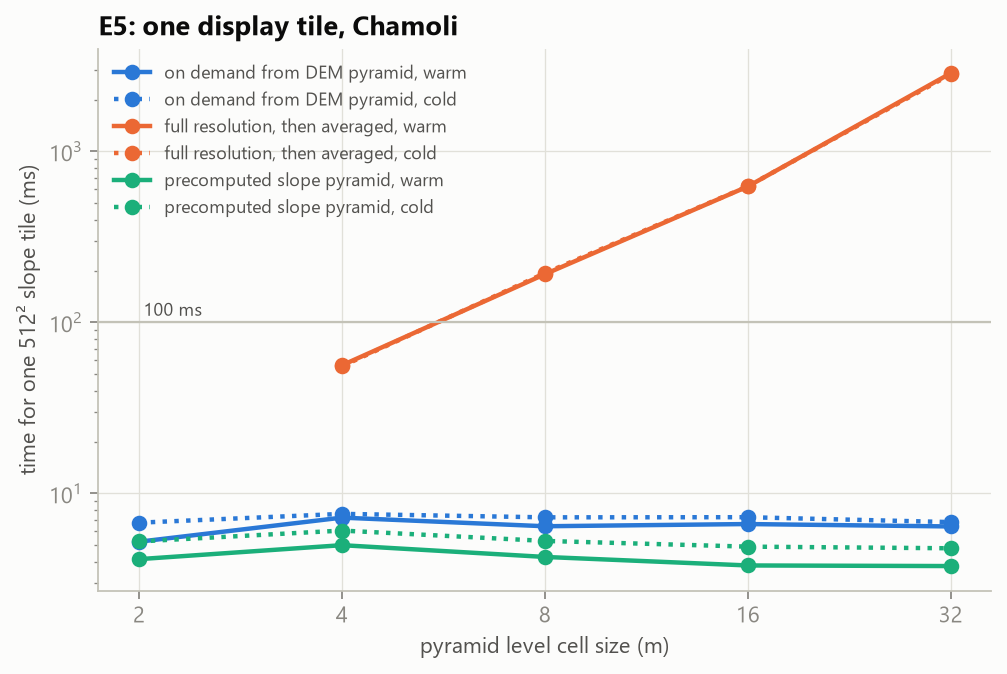
\includegraphics[width=0.49\linewidth]{e5_tile_time.png}\hfill
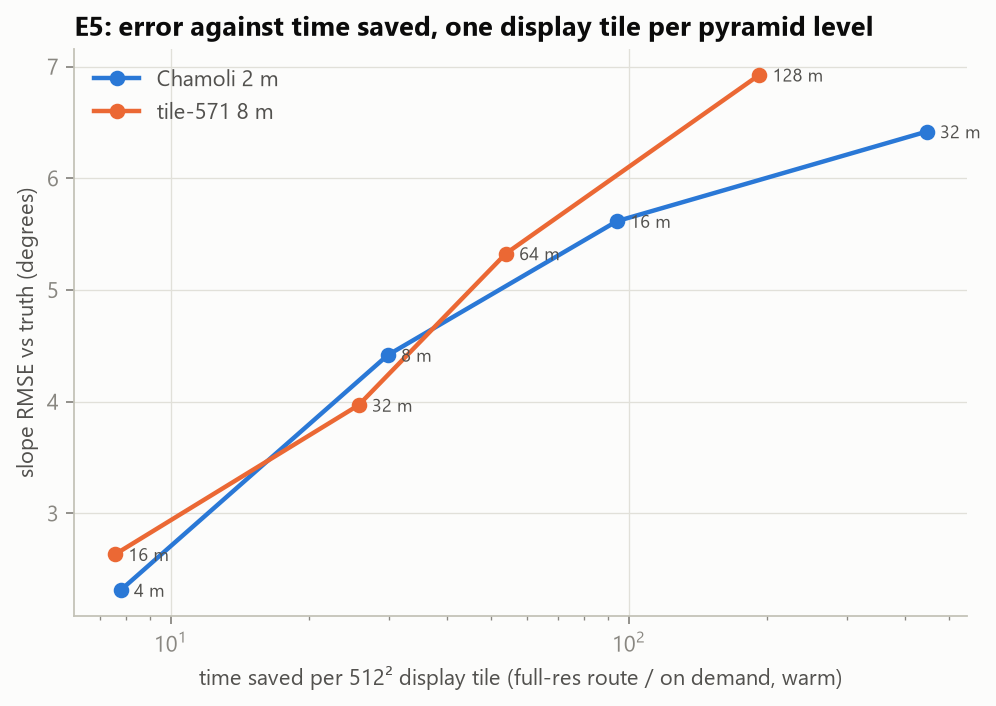
\includegraphics[width=0.49\linewidth]{e5_tradeoff.png}
\caption{Left: time for one display tile per pyramid level (Chamoli), three routes, cold and warm. Right: the G2
trade-off: slope RMSE against the time saved per tile, one point per pyramid level.}
\label{fig:e5time}
\end{figure}

\begin{itemize}
  \item \textbf{On demand costs the same at every zoom level}, 5--8\,ms per tile (Table~\ref{tab:time}): a tile
  always means reading $514^2$ cells and running the kernel on them. The exact full-resolution route reads 4$\times$
  more ground per level and grows 2--5$\times$ per level, to 2.9\,s for one tile at 32\,m. For the whole Chamoli area
  at 32\,m, on demand takes 13\,ms against 4.7\,s.
  \item \textbf{Cold or warm hardly matters} on this NVMe SSD: at most 1.5\,ms per tile for on demand.
  \item \textbf{Precomputed is 1.3--3.0\,ms faster per tile} at levels 1--4: it skips the slope kernel (about
  0.5\,ms) and the preparation of the window. On demand and precomputed both stay far below the roughly 100\,ms at
  which an interaction starts to feel slow; the full-resolution route exceeds it from two levels up.
  \item \textbf{Precomputing has a cost.} A slope pyramid built in advance is exact (apart from a small footprint
  effect of GDAL's overviews) and slightly faster per tile, but it costs a full pass for every derivative: for Chamoli 10.6\,s (1.6\,s slope, 9.0\,s compression and
  overviews) and 1005\,MB, 1.5$\times$ the DEM pyramid itself (650\,MB), because slope compresses worse than
  elevation. The ten \texttt{gdaldem} configurations would need about 10\,GB, rebuilt whenever a parameter (sun
  angle, z-factor, method) or the DEM changes. On demand needs none of it.
\end{itemize}

\subsection{Answer to Q3 (gap G2)}
Each pyramid level up saves 2--5$\times$ in time per view: 8--450$\times$ per tile for one to four levels on
Chamoli and 8--190$\times$ on the 8\,m DEM (Figure~\ref{fig:e5time}). It costs about 2.5$^\circ$ slope RMSE for the
first level and about 1.5$^\circ$ more per further level on average, as a systematic underestimate that is largest
on steep ground. Aspect costs much less (median 2--8$^\circ$). For display, the right level is the one where one
level cell is about one screen pixel: the on-demand value is then close to what that pixel should show, and every
tile costs the same few milliseconds. For analysis, slope from a coarse level should not be thresholded; the view
should be computed from full resolution (0.05--2.9\,s per tile here) or read from a precomputed slope pyramid.

%=====================================================================
\section{Interactive viewing: the system and E6}\label{sec:viewer}
E1--E5 give the design rules for a viewer: computation is cheap, decoding is the cost, and a tile computed on demand
from the right pyramid level costs the same at every zoom. This section describes the viewer we built on these rules
and measures it.

\subsection{From box zoom to continuous pan and zoom}
After E5 the team first planned a box-zoom viewer: the whole map is shown, the user drags a box, and only that box is
computed, at the level where one cell is about one screen pixel. The professor then asked for the viewer to work like
a map: pan and zoom continuously, compute only what is in view, and prefetch what the user will probably look at
next. Continuous, debounced pan and zoom became the main interaction; box zoom was kept as Shift + drag and as the
interface for QGIS. Two gates were fixed in advance:
\begin{itemize}
  \item \textbf{Gate 1:} prefetching must not raise the foreground (visible-tile) 95th-percentile (p95) latency by
  more than 10\%.
  \item \textbf{Gate 2:} the zoom debounce must reduce the tiles the server renders per zoom gesture, while the first
  frame arrives within 100\,ms of the debounce.
\end{itemize}

\subsection{Architecture}
\begin{table}[!htbp]
\centering\small
\caption{Components of the viewer system.}
\label{tab:system}
\begin{tabularx}{\linewidth}{>{\raggedright\arraybackslash}p{2.5cm}L}
\toprule
Component & Design \\
\midrule
Tile engine & Fixed $512\times512$ tile lattice per pyramid level, aligned to the COG's $512^2$ blocks, with a one-cell
halo. One tile is rendered on one thread by single-threaded Numba kernels that release Python's global interpreter
lock, so tiles run in parallel (5.4$\times$ on 8 threads). Decoded blocks are cached and shared by neighbouring tiles;
encoded tiles are cached too. Output is an 8-bit palette PNG. Modes: \emph{auto} (the level's own cells, with the E5
error), \emph{exact} (full resolution, averaged) and \emph{precomputed} (stored slope pyramid). \\
Scheduler & Foreground and background (prefetch) queues. Foreground workers are pinned to the 12 performance-core
threads, background workers to the 8 efficiency cores. Identical requests share one job; a foreground request
promotes a queued prefetch job; a newer generation of a session supersedes older work. Cancellation is checked
between read, kernel and encode. Prefetch does not start while foreground work is pending, and pauses when free
memory is low. \\
Server & FastAPI: tiles, overview, \texttt{POST /view} (a box as PNG or GeoTIFF), session generations and
statistics. Every tile reports its queue, read, decode, kernel, colour-map and encode times. A closed connection
cancels its job (median 37\,ms). \\
Web viewer & Plain JavaScript modules on a canvas. Each frame draws the needed level's tiles, falling back to a
coarser or finer cached level and then the overview. The level is the finest whose cell is at most one screen pixel
(with $\pm$10\% hysteresis). Zoom commits once, after a trailing debounce; pan requests new tiles at once. After a
commit the eight neighbouring views are prefetched, in the direction of travel first, at most two requests at a time.
Shift + drag zooms to a box. \\
QGIS plugin & Drag a box in QGIS; the server's GeoTIFF result is added as a styled layer in UTM 44N, with the level,
cell size and E5 expected error in its metadata. A full-resolution slope box is identical to \texttt{gdaldem}'s slope
of the full-resolution DEM (1.22\,M cells, maximum difference 0). \\
\bottomrule
\end{tabularx}
\end{table}

The components are listed in Table~\ref{tab:system}. The design follows directly from the earlier experiments. A
$512^2$ tile with a one-cell halo touches up to nine stored blocks, so a shared decoded-block cache brings that close
to one per tile (64 neighbouring tiles decoded 100 blocks instead of up to 576). Performance cores are kept for what
the user is waiting for, because efficiency cores are 1.7$\times$ slower. Exact tiles, which cost up to 2.9\,s at
32\,m (E5), are never prefetched. The server works within a memory budget of about 2.2\,GB. With the earlier
correctness tests, the repository has 162 automated tests.

\subsection{E6 method}
\paragraph{Virtual client.} A Python port of the viewer's policy (camera, level choice, browser cache, debounce,
generations, aborts, prefetch) reads the same policy file as the browser. It replays an interaction trace in real
time against the live server, over HTTP/1.1 with at most six connections (a browser's limit per server), and
simulates 60\,Hz frames. Python's default event-loop clock on Windows advances in 15.6\,ms steps and can fire timers
up to one step early, so the client runs its own loop on the high-resolution clock.

\paragraph{Traces.} 17 seeded traces for a $1600\times900$ view: straight and reversing pans at 0.5, 1 and 2 view
widths per second (5\,s) and a 6\,s random walk; 60\,Hz wheel bursts of 0.3, 1 and 2\,s, in and out, over 1--3
levels; ten discrete wheel notches 30--150\,ms or 120--300\,ms apart (a notched mouse wheel); 10\,s of alternating
zoom bursts and pans (zoom-pan); and three nested box zooms from the whole map to full resolution.

\paragraph{Protocol.} One factor at a time around the defaults: 24 configurations, each with 1 warm-up and 5 measured
runs per trace, 1{,}068 runs in all. Every run starts a new server process with empty caches and loads the first view
and its prefetch ring before the trace clock starts. Server counters are read at the start and end of the trace, and
memory is sampled every 50\,ms. The data is the Chamoli 2\,m DEM (levels 0--6) with hillshade, unless stated.

\paragraph{Metrics.}
\begin{itemize}
  \item \emph{Pan hit rate}: share of tiles already cached in the browser when they first enter the view while
  panning.
  \item \emph{Blank area-time}: share of view area $\times$ frames not drawn from the needed level's own tiles.
  \item \emph{TTFF} (time to first frame): last wheel tick (or end of the box animation) to the first frame showing a
  tile of the committed level. \emph{Complete}: the same to the first frame in which every visible tile is drawn.
  \item \emph{Server tiles per gesture}: foreground jobs the server finished or cancelled mid-render, per zoom
  gesture.
  \item \emph{Prefetch precision}: prefetched tiles later drawn, as a share of all prefetched tiles.
  \item \emph{Foreground p95}: measured at the client (request to response) and on the server (queue + render).
\end{itemize}

\subsection{The defaults on every trace}
\begin{table}[!htbp]
\centering\small
\caption{Default policy on every trace (median of 5 runs; debounce 200\,ms, the sweep's base). TTFF and Complete (ms)
for zoom traces include the debounce; Tiles/gest.\ = server foreground tiles per zoom gesture.}
\label{tab:base}
\footnotesize\setlength{\tabcolsep}{2pt}
\begin{tabular*}{\linewidth}{@{\extracolsep{\fill}}lrrrrrr}
\toprule
Trace & Fg req. & Prefetched & Hit rate & TTFF & Complete & Tiles/gest. \\
\midrule
pan-line 0.5/1/2 & 0/0/2 & 175/313/333 & 1.00/1.00/0.99 & & & \\
pan-reverse 0.5/1/2 & 0/0/5 & 73/128/443 & 1.00/1.00/0.98 & & & \\
pan-walk & 0 & 290 & 1.00 & & & \\
zoom in 0.3/1/2\,s & 20/15/20 & & & 272/273/289 & 325/325/358 & 20/15/20 \\
zoom out 0.3/1/2\,s & 18/20/12 & & & 269/264/257 & 321/314/276 & 18/20/12 \\
zoom-pan & 36 & 128 & 1.00 & 206 & 206 & 7.2 \\
box & 35 & 125 & & 64 & 127 & \\
\bottomrule
\end{tabular*}
\end{table}

On-the-fly computation keeps up with continuous viewing (Table~\ref{tab:base}):
\begin{itemize}
  \item \textbf{Pans} need almost no foreground requests: the prefetch ring already holds the tiles.
  \item \textbf{Zoom bursts:} the first exact tile arrives 57--89\,ms after the commit, and the full view 76--158\,ms
  after it.
  \item \textbf{Box zoom} shows its first exact tile 64\,ms after the animation ends, and the whole view after
  127\,ms.
  \item \textbf{Cost:} the server never needed more than 982\,MiB, and prefetch used about 3 CPU-seconds of the
  efficiency cores per 5\,s pan.
\end{itemize}
During zoom-pan, the needed level's own tiles cover the whole view except for a few hundred milliseconds after each
zoom-in, when cached coarser tiles stand in.

\subsection{Debounce (gate 2)}

\begin{itemize}
  \item \textbf{Without a debounce} every wheel tick commits, up to 121 times in a 2\,s burst. The server renders a
  median of 62 foreground tiles per gesture and cancels 4--19 of them mid-render.
  \item \textbf{With a debounce} it renders 19, \textbf{3.3$\times$ fewer}, and the first exact tile arrives
  63--71\,ms after the debounce fires (Table~\ref{tab:debounce}, Figure~\ref{fig:debounce}). Gate 2 passes.
  \item \textbf{Notched wheels decide the value.} At 60\,Hz the ticks are 17\,ms apart, so every debounce from 100
  to 250\,ms behaves the same. A notched mouse wheel, with gaps of 30--300\,ms, separates them: 100\,ms commits
  between notches and does as badly as no debounce (36 tiles), while 150\,ms and longer coalesce the gesture
  (15 tiles). 200\,ms only adds 40--50\,ms of delay over 150\,ms, so the default became 150\,ms.
  \item \textbf{A forced commit} after 500\,ms of continuous scrolling almost doubles the tiles (35 against 19) for
  9\,ms less delay, so it stays off.
\end{itemize}

\begin{table}[!htbp]
\centering\small
\caption{Server foreground tiles per zoom gesture and delay, by debounce (medians).}
\label{tab:debounce}
\begin{tabularx}{\linewidth}{lRRRRR}
\toprule
Debounce & 60\,Hz bursts & Notched 30--150\,ms & Notched 120--300\,ms & TTFF $-$ debounce, bursts (ms) & TTFF, bursts (ms) \\
\midrule
off (every tick) & 62 & 36 & 48 & -- & 6 \\
100\,ms & 19 & 36 & 48 & 63 & 163 \\
\textbf{150\,ms (new default)} & 19 & \textbf{15} & \textbf{39} & 68 & 218 \\
200\,ms & 19 & 15 & 39 & 71 & 271 \\
250\,ms & 19 & 15 & 39 & 68 & 318 \\
200\,ms + forced commit at 500\,ms & 35 & 30 & 39 & 62 & 262 \\
\bottomrule
\end{tabularx}
\end{table}

\begin{figure}[!htbp]
\centering
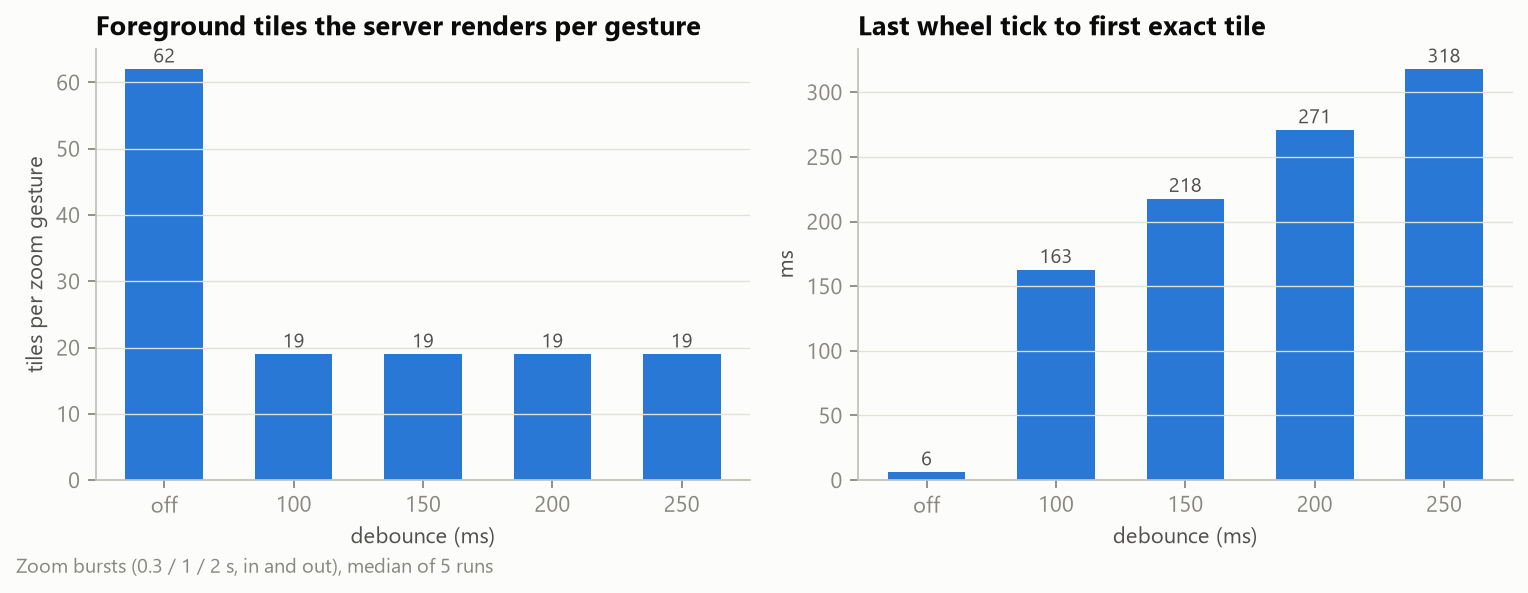
\includegraphics[width=0.9\linewidth]{e6_debounce.png}
\caption{Zoom bursts at 60\,Hz: foreground tiles the server renders per gesture, and time from the last tick to the
first exact tile, against the debounce.}
\label{fig:debounce}
\end{figure}

\subsection{Prefetch and its effect on the foreground (gate 1)}
\begin{table}[!htbp]
\centering\small
\caption{Prefetch policies over the seven pan traces and zoom-pan (40 runs each; median [interquartile range]).}
\label{tab:prefetch}
\begin{tabularx}{\linewidth}{Lrrrr}
\toprule
Policy & Foreground requests & Pan hit rate & Prefetched & Precision \\
\midrule
prefetch off & 104 [68--135] & 0.30 [0.00--0.51] & 0 & -- \\
defaults (back-off at p95 $>$ 250\,ms) & 0 [0--4] & 1.00 [1.00--1.00] & 218 & 0.34 \\
first policy (back-off at 100\,ms) & 0 [0--56] & 1.00 [0.70--1.00] & 192 & 0.29 \\
no back-off & 0 [0--4] & 1.00 [1.00--1.00] & 232 & 0.34 \\
ring in fixed order & 0 [0--7] & 1.00 [0.97--1.00] & 292 & 0.33 \\
\bottomrule
\end{tabularx}
\end{table}

\begin{figure}[!htbp]
\centering
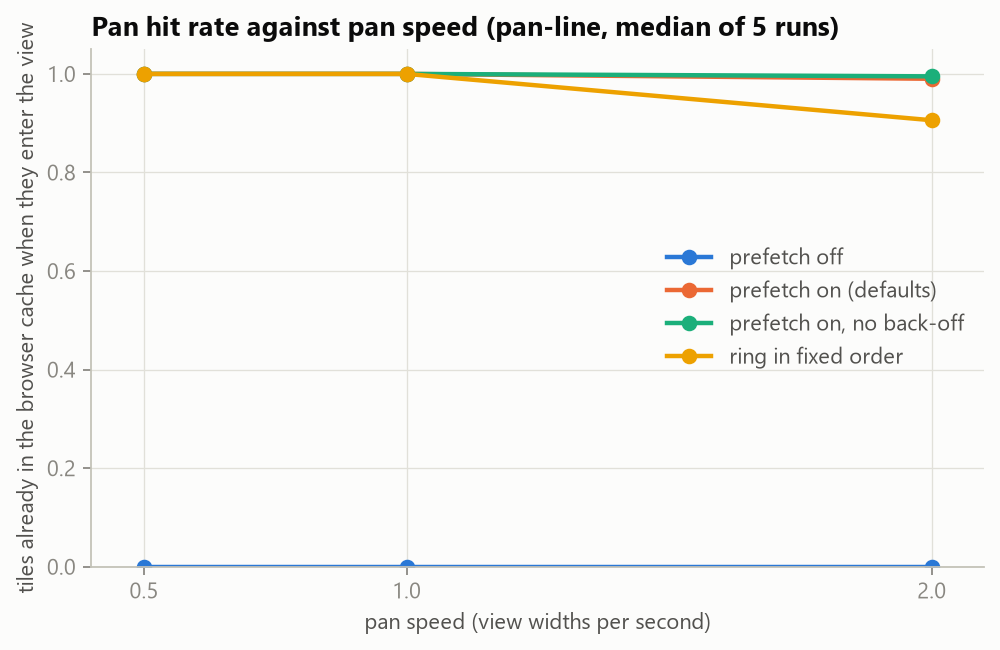
\includegraphics[width=0.44\linewidth]{e6_hit_vs_speed.png}
\caption{Share of tiles already in the browser when they enter the view, straight pans, by pan speed.}
\label{fig:hit}
\end{figure}

\begin{itemize}
  \item \textbf{With prefetch}, 98--100\% of the tiles entering the view during a pan are already cached, at every
  speed. The pans need 0--5 foreground requests instead of 36--202 (Table~\ref{tab:prefetch},
  Figure~\ref{fig:hit}).
  \item \textbf{Without prefetch} the hit rate is 0\% on a straight pan and about 50\% when the pan turns back. The
  view still looks almost complete (blank area-time 0.2--3.4\%), because each new tile arrives in about 50\,ms and a
  coarser level covers the gap.
  \item \textbf{Cost:} the ring fetches 2--5 tiles for each one used (precision 0.20--0.56), because it always loads
  directions the user does not take.
  \item \textbf{Ordering:} loading the direction of travel first keeps the hit rate at 0.99 at two view widths per
  second; a fixed order drops it to 0.91.
  \item \textbf{Back-off threshold:} the first policy stopped prefetch for 2\,s whenever the foreground p95 exceeded
  100\,ms. That is the cold-start latency, so prefetch switched off at random, and the fast reversing pan fell to a
  0.50 hit rate. At 250\,ms the policy matches ``no back-off'' on every trace and keeps a safety valve.
\end{itemize}

\begin{figure}[!htbp]
\centering
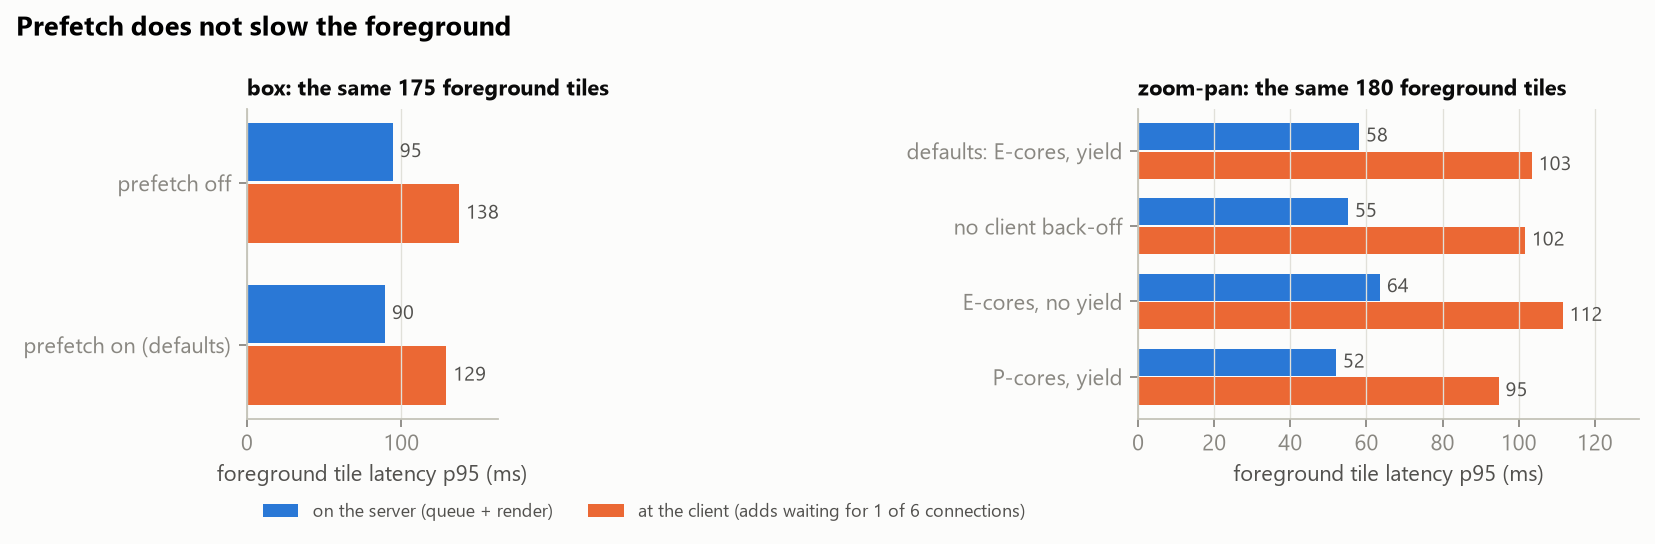
\includegraphics[width=0.92\linewidth]{e6_fg_p95.png}
\caption{Foreground tile latency (95th percentile) on identical tile sets: on the server (queue + render) and at the
client (which also waits for one of six connections).}
\label{fig:fg}
\end{figure}

\paragraph{Gate 1.} The gate as first written compares foreground p95 per trace with prefetch on and off. That
compares different tiles: with prefetch on, pans need almost no foreground tiles, and what remains are cold tiles at a
new level. The like-for-like test is the box trace, where the foreground tiles are identical (Figure~\ref{fig:fg}):
\begin{itemize}
  \item \textbf{Result:} server p95 is 90\,ms with prefetch and 95\,ms without; client p95 is 129 against 138\,ms.
  Prefetch is slightly faster, because it has already decoded shared blocks. Gate 1 passes.
  \item \textbf{Why:} prefetch stops at the first input event of a gesture and restarts only once the view is
  complete. Only 25 of 905 foreground tiles (3\%) were ever requested while a prefetch request was in flight.
  \item \textbf{Placement:} letting prefetch start while foreground work is pending raises server p95 by 9\% on
  zoom-pan (64 against 58\,ms).
  \item \textbf{Pinning held throughout:} 20{,}242 foreground jobs ran on performance cores only, and 122{,}215
  prefetch jobs on efficiency cores only.
\end{itemize}

\subsection{Workers, caches, products and data}
\begin{table}[!htbp]
\centering\small
\caption{Mixed traces (pan-walk, zoom-pan, two bursts, box; 25 runs each; medians).}
\label{tab:mixed}
\begin{tabularx}{\linewidth}{lRRRRR}
\toprule
Configuration & Client p95 (ms) & Server p95 (ms) & Complete (ms) & Blocks decoded & Peak RSS (MiB) \\
\midrule
defaults (8 workers, 1024\,MiB block cache) & 104 & 98 & 260 & 185 & 608 \\
4 / 6 foreground workers & 106 / 101 & 76 / 92 & 254 / 251 & 185 & 588 / 598 \\
no block cache & 146 & 111 & 285 & 1{,}128 & 386 \\
256\,MiB block cache & 108 & 94 & 260 & 185 & 608 \\
result cache off & 103 & 91 & 257 & 185 & 576 \\
slope / aspect & 115 / 115 & 97 / 103 & 255 / 258 & 185 & 606 / 608 \\
precomputed slope & 93 & 56 & 248 & 160 & 562 \\
HMA 8\,m DEM & 118 & 92 & 268 & 130 & 594 \\
OS file cache flushed & 103 & 104 & 257 & 185 & 608 \\
\bottomrule
\end{tabularx}
\end{table}

\begin{itemize}
  \item \textbf{The browser's six connections set the foreground latency.} The client sees about 40\,ms more than the
  server at p95, because tiles wait for a connection. 4, 6 or 8 foreground workers give the same client latency
  (Table~\ref{tab:mixed}); 8 are kept so that a second client such as QGIS does not queue.
  \item \textbf{The block cache matters:} without it the server decodes 6$\times$ more blocks and the client p95 rises
  40\%. 256\,MiB suffices for these short traces.
  \item \textbf{The result cache} has no effect within a single fresh session, where no tile is asked for twice; it
  serves repeat visits and several clients.
  \item \textbf{Product, mode and data hardly matter.} Slope and aspect are about 10\% slower than hillshade.
  Precomputed slope is fastest on the server (no halo, no kernel). The 8\,m DEM behaves like the 2\,m one.
  \item \textbf{A flushed OS cache changes nothing:} decoding, not the disk, is the cost, as in E1--E5.
\end{itemize}

\paragraph{A real browser.} The same traces replayed in headless Chrome, driven in real time over the DevTools
protocol, gave the same commits, foreground requests (15, 0 and 35) and prefetched tiles as the virtual client,
view-complete times within 10\% (298 against 325\,ms; 123 against 127\,ms), and first frames 18--25\,ms sooner. The
simulated latencies are therefore slight upper bounds.

\subsection{Policy chosen from the data, and answer to Q4}
Table~\ref{tab:policy} lists the settings chosen from these results. Computing derivatives on demand keeps up with continuous pan and zoom on one laptop.
Panning is seamless with a velocity-first ring of neighbouring views, at no cost to the foreground, because prefetch
never runs while the user is waiting. A 150\,ms trailing debounce cuts the server's work per zoom gesture
3.3$\times$, and the first exact tile follows within about 70\,ms. The latency that remains comes from the browser's
connection limit and from decoding compressed blocks, not from computing slope or hillshade.

\begin{table}[!htbp]
\centering\small
\caption{Viewer settings before and after E6.}
\label{tab:policy}
\begin{tabularx}{\linewidth}{>{\raggedright\arraybackslash}p{2.9cm}>{\raggedright\arraybackslash}p{2.5cm}>{\raggedright\arraybackslash}p{2.5cm}L}
\toprule
Setting & Before & After & Reason \\
\midrule
Zoom debounce & 200\,ms & \textbf{150\,ms} & Same tiles as 200 and 250\,ms on every trace; 40--50\,ms sooner; 100\,ms commits
between notches \\
Forced commit & off & off & Nearly doubles tiles per gesture for 9\,ms \\
Prefetch back-off & 100\,ms & \textbf{250\,ms} & 100\,ms sits at the cold-start p95 and switches prefetch off at random \\
Prefetch order & velocity-first & velocity-first & 0.99 against 0.91 hit rate at two view widths per second \\
Prefetch in flight & 2 & 2 & Leaves 4 of the 6 connections for the foreground \\
Foreground workers & 8 & 8 & 4--8 equal for one browser; 8 leave room for a second client \\
Prefetch placement & E-cores + yield & E-cores + yield & Not yielding costs 9\% foreground p95 \\
Block cache & 1024\,MiB & 1024\,MiB & 256\,MiB suffices for short traces; longer sessions reuse more \\
\bottomrule
\end{tabularx}
\end{table}

%=====================================================================
\section{Discussion}\label{sec:discussion}
\subsection{The bottleneck across the project}
Table~\ref{tab:bottleneck} brings the stage measurements of all experiments together. The same pattern runs through
them: arithmetic is never the limit for long. Once computation is parallel, the time goes to decompressing,
copying and writing data, and in display to reading data at the wrong resolution.

\begin{table}[!htbp]
\centering\small
\caption{The limiting stage of each tool or route, as measured.}
\label{tab:bottleneck}
\begin{tabularx}{\linewidth}{>{\raggedright\arraybackslash}p{3.6cm}>{\raggedright\arraybackslash}p{4.4cm}L}
\toprule
Tool or route & Limiting stage & Evidence \\
\midrule
\texttt{gdaldem}, whole grid & single-threaded computation & 73\% of run time; 0.99 of 22 threads (E1) \\
QGIS, no pyramid & reading full-resolution data & 31.9\,s per redraw at 1\,m, about 12.7\,GB read (QGIS) \\
CPU engine, whole grid & writing; without output, decompression & writer busy 65.3\,s of 68.2\,s; read wait 22.9\,s
without output (E3) \\
GPU engine, whole grid & decompression, then writing & read wait 25.7\,s; with 8 readers the writer wait is 30.6\,s
(E4) \\
GPU kernel & copies over PCIe & 95\% of GPU time for a $2048^2$ window (E4) \\
Tile on demand & reading and decoding blocks & 5--8\,ms per tile, of which the kernel is about 0.5\,ms (E5) \\
Viewer & browser connections, block decoding & client p95 about 40\,ms above server; no block cache:
6$\times$ blocks, +40\% p95 (E6) \\
\bottomrule
\end{tabularx}
\end{table}

\paragraph{G1.} Standard GDAL/QGIS tools do not break on a 16\,GB laptop, even at 10.8 billion cells; they become
slow. Processing is limited by single-threaded computation and display by reading full-resolution data. Only the
naive approach of loading the whole grid fails, at roughly 0.5--0.7 billion cells. Parallel computation moves the
bottleneck to decompression and writing, and a GPU moves it further to PCIe copies and the disk write. Our
answer to the professor's question ``where is the actual bottleneck?'' is therefore: it depends on the tool, and
after each fix it is data movement.

\paragraph{G2.} Computing derivatives on demand from the pyramid makes every view cost the same few milliseconds,
whatever the zoom: 8--450$\times$ cheaper per tile than an exact computation from full resolution, and with none of
the storage that precomputed products need. The cost is a known, measured underestimate of slope: about 2.5$^\circ$
RMSE one level up and about 1.5$^\circ$ more per further level, largest on steep terrain.

\paragraph{Comparison with the literature.} Our results agree with the literature that data movement limits large
raster processing more than arithmetic, but with a twist: on an NVMe SSD the disk itself is not the slow part.
Decompression and writing are. This is close to the finding of Sanchez-Fernandez et al.\ \cite{sanchez} that the
memory layout mattered more than adding GPUs. Like Yu et al.\ \cite{yu}, we find that the CPU and the GPU each suit
part of the work: in our case the CPU for small windows and the GPU from $512^2$ cells, or for fused products. For
display, our results confirm the pyramid approach of Losasso and Hoppe \cite{clipmaps} and Campos et al.\
\cite{campos} and extend it from elevation to derived products computed on demand.

\subsection{Practical recommendations}
\begin{enumerate}
  \item \textbf{Store DEMs as tiled COGs} with 512 tiles, ZSTD compression and internal averaging overviews. Avoid
  LZW. GDAL's overviews can be used as a pyramid even when the grid size is not a power of two.
  \item \textbf{For whole-grid processing}, stream the grid in windows; never load it whole beyond about half a
  billion cells on 16\,GB. Use a compiled parallel kernel on the performance cores (12 threads beat 22), 2048-cell
  windows, and fuse products that share a gradient. Use the GPU when available for fused products
  (1.4--1.7$\times$ over the CPU engine on the large grids), but expect the next gains from I/O, not from faster
  kernels.
  \item \textbf{For display, always use a pyramid}, choose the level where one cell is about one screen pixel, and
  compute derivatives on demand. Precompute only the one or two most used products, if storage allows. Cache
  decoded blocks: decoding, not computing, is the main cost of a tile.
  \item \textbf{For analysis, do not threshold slope from a coarse level.} Compute the view from full resolution or
  read a precomputed slope pyramid, and show the expected error of the level in use.
  \item \textbf{For interaction}, use a trailing zoom debounce of about 150\,ms, prefetch the neighbouring views in
  the direction of travel on the efficiency cores, let prefetch yield to foreground work, keep prefetch to two
  connections, and set any latency back-off well above the cold-start latency.
  \item \textbf{For benchmarking on a hybrid-core laptop}, pin processes to one core class, verify cold caches, and
  watch for background scanning of large outputs.
\end{enumerate}

\subsection{Limitations}
\begin{itemize}
  \item \textbf{One laptop.} All timings are for one machine with a local NVMe SSD. Ratios (speed-ups, stage shares)
  transfer better than absolute times. A network-hosted COG would add latency per request and widen the gap between
  the E5 routes.
  \item \textbf{Synthetic grids} at 2\,m and 1\,m add cells but no terrain detail; they are used only for timing.
  On the synthetic grids warm values are single runs.
  \item \textbf{One region of steep terrain} (mean true slope 38$^\circ$ on Chamoli and 31$^\circ$ on the 8\,m area).
  Flatter regions would show smaller pyramid errors; the per-class tables carry over. The truth is itself a DEM with
  its own noise, and the 8\,m DEM's truth is only 8\,m.
  \item \textbf{Only GDAL and QGIS} were used as the baseline; other tools such as WhiteboxTools, GRASS or
  xarray-spatial were not benchmarked.
  \item \textbf{E6 covers one client} with short, seeded traces (1--11\,s) and a cold server. Caches never fill, so
  long sessions, several clients and returning users are not measured. The virtual client agrees with a real browser
  on three traces.
  \item \textbf{The viewer runs on the CPU only.} By E4, a $512^2$ tile is at the CPU/GPU crossover (0.54\,ms on
  the CPU against 0.41\,ms on the GPU with copies), so the GPU would gain little per tile.
  \item \textbf{Python start-up} (about 0.5\,s) is included in every engine run, just as \texttt{gdaldem}'s start-up
  is; it dominates the small grids.
\end{itemize}

\subsection{Future work}
\begin{itemize}
  \item \textbf{Gap G3:} viewshed (exact R3 against approximate XDraw and \texttt{gdal\_viewshed}: time and the share
  of cells classified differently in high relief, after converting heights to one vertical datum) and terrain
  distance (Dijkstra against A* on a slope-based cost surface).
  \item \textbf{A GPU tile path} as an E6 variant, and GPU use where computation is a large share (fused products,
  heavier operators).
  \item \textbf{A Cesium globe} that drapes the viewer's tiles over 3D terrain, as discussed in the meeting.
  \item \textbf{Several clients and long sessions}, with traces recorded from people, to measure the result cache,
  evictions and a returning user.
  \item \textbf{A per-level correction factor} for the systematic slope underestimate, which could remove most of
  the bias but not the spread.
  \item \textbf{Batch I/O}: keep the halo rows of the previous window or share decoded tiles between readers, write
  compressed output with spare cores, and test network-hosted COGs.
  \item \textbf{A QGIS drawing baseline} for the same boxes as the plugin, which was planned for E6 but not run.
\end{itemize}

%=====================================================================
\section{Conclusion}\label{sec:conclusion}
We set out to find how far very large, high-resolution DEMs can be processed and displayed on one laptop, and where
the bottleneck really is. Standard tools do not run out of memory, even on a 43\,GB grid; they are slow, because
\texttt{gdaldem} computes on one thread and QGIS without a pyramid reads full-resolution data. Our own tiled engine
removes the computation bottleneck on the CPU (2.1--3.5$\times$ faster, identical results, flat memory) and on the
GPU (a 50$\times$ faster kernel), and in doing so shows that the real limit is data movement: decompression, PCIe
copies and writing. The way past that limit is not to process everything. Computing derivatives on demand from the
right pyramid level costs 5--8\,ms per tile at every zoom, 8--450$\times$ less than an exact computation, at a
measured price of about 2.5$^\circ$ slope RMSE one level up and about 1.5$^\circ$ more per further level. A viewer built
on this principle keeps up with continuous pan and zoom on the laptop, with seamless panning, a 150\,ms debounce
that cuts the server's work per zoom 3.3$\times$, and prefetching that never slows what the user is looking at.

%=====================================================================
\phantomsection\addcontentsline{toc}{section}{References}
\begin{thebibliography}{99}\footnotesize\setlength{\itemsep}{1pt}
\bibitem{amatulli} Amatulli, G., McInerney, D., Sethi, T., Strobl, P., \& Domisch, S. (2020). Geomorpho90m,
empirical evaluation and accuracy assessment of global high-resolution geomorphometric layers. \emph{Scientific
Data}, 7, 162.
\bibitem{barnes} Barnes, R. (2016). Parallel Priority-Flood depression filling for trillion cell digital elevation
models on desktops or clusters. \emph{Computers \& Geosciences}, 96, 56--68.
\bibitem{chamoli} Bhushan, S., \& Shean, D. (2021). Chamoli Disaster Pre-event 2-m DEM Composite: September 2015.
Zenodo. doi:10.5281/zenodo.4554647.
\bibitem{campos} Campos, R., Quintana, J., Garcia, R., Schmitt, T., Spoelstra, G., \& Schaap, D.\,M.\,A. (2020). 3D
simplification methods and large scale terrain tiling. \emph{Remote Sensing}, 12(3), 437.
\bibitem{cauchi} Cauchi-Saunders, A.\,J., \& Lewis, I.\,J. (2015). GPU enabled XDraw viewshed analysis.
\emph{Journal of Parallel and Distributed Computing}, 84, 87--93.
\bibitem{deng} Deng, Y., Wilson, J.\,P., \& Bauer, B.\,O. (2007). DEM resolution dependencies of terrain attributes
across a landscape. \emph{International Journal of Geographical Information Science}, 21(2), 187--213.
\bibitem{dou} Dou, W., Li, Y., \& Wang, Y. (2019). An equal-area triangulated partition method for parallel Xdraw
viewshed analysis. \emph{Concurrency and Computation: Practice and Experience}, 31(17), e5216.
\bibitem{cop30} European Space Agency (2021). Copernicus Global Digital Elevation Model (GLO-30). Distributed by
OpenTopography. doi:10.5069/G9028PQB.
\bibitem{guth} Guth, P.\,L., \& Kane, M. (2021). Slope, aspect, and hillshade algorithms for non-square digital
elevation models. \emph{Transactions in GIS}, 25(5), 2309--2332.
\bibitem{hart} Hart, P.\,E., Nilsson, N.\,J., \& Raphael, B. (1968). A formal basis for the heuristic determination
of minimum cost paths. \emph{IEEE Transactions on Systems Science and Cybernetics}, 4(2), 100--107.
\bibitem{ho} Ho, Y.-F., Grohmann, C.\,H., Lindsay, J., Reuter, H.\,I., Parente, L., Witjes, M., \& Hengl, T.
(2025). GEDTM30: Global ensemble digital terrain model at 30\,m and derived multiscale terrain variables.
\emph{PeerJ}, 13, e19673.
\bibitem{horn} Horn, B.\,K.\,P. (1981). Hill shading and the reflectance map. \emph{Proceedings of the IEEE},
69(1), 14--47.
\bibitem{numba} Lam, S.\,K., Pitrou, A., \& Seibert, S. (2015). Numba: A LLVM-based Python JIT compiler.
\emph{Proc.\ Second Workshop on the LLVM Compiler Infrastructure in HPC}, 1--6.
\bibitem{clipmaps} Losasso, F., \& Hoppe, H. (2004). Geometry clipmaps: Terrain rendering using nested regular
grids. \emph{ACM Transactions on Graphics}, 23(3), 769--776.
\bibitem{cupy} Okuta, R., Unno, Y., Nishino, D., Hido, S., \& Loomis, C. (2017). CuPy: A NumPy-compatible library
for NVIDIA GPU calculations. \emph{Workshop on Machine Learning Systems (LearningSys), NIPS 2017}.
\bibitem{polidori} Polidori, L., \& El Hage, M. (2020). Digital elevation model quality assessment methods: A
critical review. \emph{Remote Sensing}, 12(21), 3522.
\bibitem{riley} Riley, S.\,J., DeGloria, S.\,D., \& Elliot, R. (1999). A terrain ruggedness index that quantifies
topographic heterogeneity. \emph{Intermountain Journal of Sciences}, 5(1--4), 23--27.
\bibitem{sanchez} Sanchez-Fernandez, A.\,J., Romero, L.\,F., Bandera, G., \& Tabik, S. (2021). A data relocation
approach for terrain surface analysis on multi-GPU systems: A case study on the total viewshed problem.
\emph{International Journal of Geographical Information Science}, 35(8), 1500--1520.
\bibitem{hma8} Shean, D. (2017). High Mountain Asia 8-meter DEM Mosaics Derived from Optical Imagery, Version 1.
NASA NSIDC DAAC. doi:10.5067/KXOVQ9L172S2.
\bibitem{trevisani} Trevisani, S., Teza, G., \& Guth, P.\,L. (2023). Hacking the topographic ruggedness index.
\emph{Geomorphology}, 439, 108838.
\bibitem{wilson} Wilson, M.\,F.\,J., O'Connell, B., Brown, C., Guinan, J.\,C., \& Grehan, A.\,J. (2007).
Multiscale terrain analysis of multibeam bathymetry data for habitat mapping on the continental slope.
\emph{Marine Geodesy}, 30(1--2), 3--35.
\bibitem{yu} Yu, Z., Zhou, C., \& Li, M. (2024). A parallel strategy to accelerate neighborhood operation for
raster data coordinating CPU and GPU. \emph{Cartography and Geographic Information Science}, 51(6), 813--829.
\bibitem{zt} Zevenbergen, L.\,W., \& Thorne, C.\,R. (1987). Quantitative analysis of land surface topography.
\emph{Earth Surface Processes and Landforms}, 12(1), 47--56.
\bibitem{zhang} Zhang, W., \& Montgomery, D.\,R. (1994). Digital elevation model grid size, landscape
representation, and hydrologic simulations. \emph{Water Resources Research}, 30(4), 1019--1028.
\end{thebibliography}

%=====================================================================
\appendix
\section{Reproducibility}
The code, scripts, traces and results are in the project repository; the raster data are kept outside it and listed
with checksums in \texttt{datasets/manifest.csv}. The commands below rebuild the data and rerun the experiments (Python environment \texttt{geo}, from the repository root); Table~\ref{tab:repo} gives the layout.

\begin{footnotesize}
\begin{verbatim}
python datasets/prepare.py --synthetic                          # all grids
powershell -ExecutionPolicy Bypass -File bench\run_phase2.ps1   # E1, E2, QGIS
powershell -ExecutionPolicy Bypass -File bench\run_e3.ps1       # E3 (CPU)
powershell -ExecutionPolicy Bypass -File bench\run_e4.ps1       # E4 (GPU)
python -m bench.experiments.e4_crossover                        # GPU crossover
python -m bench.experiments.e5_timing --precompute              # slope pyramids
python -m bench.experiments.e5_accuracy                         # E5 accuracy
powershell -ExecutionPolicy Bypass -File bench\run_e5.ps1       # E5 timing
powershell -ExecutionPolicy Bypass -File bench\run_e6.ps1       # E6 sweep
python -m bench.e6_browser                                      # Chrome check
python -m pytest tests/ -q                                      # unit tests
python -m tests.check_full_grid                                 # every cell
python -m bench.analysis.phase2_report     # also phase3_report, e4_report,
                                           # e5_report, e6_report, run_stats
python -m server                           # viewer: http://127.0.0.1:8765/viewer/
\end{verbatim}
\end{footnotesize}

\begin{center}\begin{minipage}{\linewidth}\centering\small
\captionsetup{type=table}\caption{Repository layout.}
\label{tab:repo}
\begin{tabularx}{\linewidth}{>{\raggedright\arraybackslash}p{4.2cm}L}
\toprule
Folder & Contents \\
\midrule
\texttt{datasets/} & download and preparation scripts, data manifest \\
\texttt{demlab/} & engine (pipeline, CPU and CUDA kernels), pyramid helpers, tile engine, caches, scheduler \\
\texttt{server/}, \texttt{viz/web/} & FastAPI tile server and web viewer \\
\texttt{qgis\_plugin/} & QGIS plugin with install notes \\
\texttt{bench/} & harness, experiment drivers E1--E6, virtual client, traces, analysis scripts \\
\texttt{tests/} & unit tests and the full-grid correctness check \\
\texttt{results/} & every run (\texttt{runs.csv}, \texttt{e5\_*.csv}, \texttt{e6\_*.csv}), tables, charts, run spreads \\
\texttt{docs/} & project plan and the detailed results of each phase \\
\bottomrule
\end{tabularx}
\end{minipage}\end{center}

\section{Problems met and how they were solved}
Several results above depend on problems found during the work. Table~\ref{tab:problems} lists the main ones.

\begin{center}\begin{minipage}{\linewidth}\centering\small
\captionsetup{type=table}\caption{Main problems and their fixes.}
\label{tab:problems}
\begin{tabularx}{\linewidth}{>{\raggedright\arraybackslash}p{7.2cm}L}
\toprule
Problem & Fix or lesson \\
\midrule
No free 1\,m DEM for the region & Cubic synthetic grids, tested to time like real data; used for timing only \\
Unpinned runs on a hybrid CPU (one run 2$\times$ slower) & Pin every tool to the performance cores \\
Defender scanning 10--40\,GB outputs; deleted files kept their space (108\,GB filled the disk) & Exclude only the
scratch folders; wait for freed space between runs; re-run everything \\
A ``read'' reference that also computed a checksum & A pure read-and-decompress reference \\
Engine submitted all window reads at once (up to $\sim$86\,GB at 1\,m) & At most six windows in flight \\
Writing in the compute thread blocked the kernel & One dedicated writer thread \\
Mismatch with \texttt{gdaldem} on nearly flat cells & \texttt{gdaldem} sums in float32; reproduced to prove equality \\
Small windows unexpectedly slow & The halo re-decodes neighbouring tiles; 2048 windows \\
Straightforward GPU port slower than the CPU & Own CUDA kernel, pinned memory, two streams \\
GDAL overviews are not exact halvings & Footprints from geometry; exact-pyramid cross-check \\
Client timers fired up to 16\,ms early (Windows clock) & First E6 attempt stopped; client on a high-resolution
loop \\
Gate 1 as written compared different tiles & Like-for-like comparison on the box trace \\
60\,Hz traces could not choose the debounce & Notched-wheel traces added \\
Headless Chrome's virtual time distorted latencies & Real-time Chrome over the DevTools protocol \\
\bottomrule
\end{tabularx}
\end{minipage}\end{center}


\end{document}
